\documentclass[a4paper,11pt,titlepage]{article}
\usepackage[a4paper]{geometry}
\usepackage{listings}
\usepackage{textcomp}
\usepackage{color}
\usepackage{graphicx}
\usepackage{epsfig}
\usepackage{latexsym}
\usepackage[utf8]{inputenc}
\usepackage{longtable}
\usepackage{enumitem}
\usepackage{wrapfig}
\usepackage{amsmath}
\usepackage{amsfonts}
\usepackage{amssymb}
\usepackage{tabu}
\usepackage{url}
\graphicspath{ {drafts/images/} }
\definecolor{dkgreen}{rgb}{0,0.6,0}
\definecolor{gray}{rgb}{0.5,0.5,0.5}
\definecolor{mauve}{rgb}{0.58,0,0.82}
\lstset{frame=tb,
  language=Java,  
  showstringspaces=false,
  columns=flexible,
  basicstyle={\small\ttfamily},
  numbers=none,
  numberstyle=\tiny\color{gray},
  keywordstyle=\color{blue},
  commentstyle=\color{dkgreen},
  stringstyle=\color{mauve},
  breaklines=true,
  breakatwhitespace=true,
  tabsize=3
}
\begin{document}
\title{LondonSW: Traffic Simulator}
\author{Violetta Avkhukova\\Felix Santiago Anda Basabe\\Rawan Mohammed Alrahili\\Jia Liu\\Yakubu Aliyu Doma}
\maketitle

\part{Introduction}
\paragraph{}
As population grows as a result of rapid development of cities, so does the volume of traffic and congestion. Managing traffic congestion is a serious issue, and  with the ever-increasing volume of traffic, this problem is expected to get worse.
\paragraph{}
A simple description of traffic congestion is given as a situation where the volume of traffic surpasses the capacity of the road. However, the Department for Transport provide a more quantifiable description of congestion as "the average delay experienced for each kilometre travelled compared to driving at speeds typical when traffic is light" \cite{2}.
\paragraph{}
A lot of attention has been given to modelling and simulation of traffic flows to determine the causes of traffic congestion, to determine the effectiveness of traffic policies, and how such road policies can be improved and also aid in the development and design or road infrastructures.

\section{Problem Definition}
\paragraph{}
Many strategies have been proposed and implemented with the primary objective of relieving congestion. However, these strategies have varying effects and it is not always self-evident which strategy works best for a given scenario. A straightforward strategy is to construct new roads to increase the road capacity or improve already existing roads, but  this rarely serves as a long time solution.
\paragraph{}
Congestion is described as self managing, that is; as the capacity of the road increases, so does the traffic demand to fill the new capacity. This notion is described as Pigou-Knight analysis, which suggests improving road network capacity does not guarantee reduced congestion, on the contrary it can be counter-productive by making congestion worse \cite{1,2}. This strategy regarded as one of the most expensive ways of dealing with congestion \cite{2}.
\paragraph{}
Traffic simulation is important because it allows very complex traffic models to be studied and analysed. In situations where evaluating analytical and numerical data is not sufficient enough it provides visual description, of both existing and future scenarios. Another huge importance of traffic simulation is, it enables us see the outcome changes to road infrastructure will have.

\section{Project Summary}
\paragraph{}
In this report, we give a detailed documentation of the process involved in developing a traffic simulation software. Our traffic simulation software consist of two parts: the simulation environment and the map builder. 
\paragraph{}
The first part of the system is the simulation environment where actual simulation runs. This part allows a user to load a map and run a simulation on it with some number of vehicles. 
\paragraph{}
The second part of the system is the map making mode. This part of our system allows the user to create a map. That is, it serves as an interface which provides all the necessary functionalities for designing road infrastructure (i.e lanes, intersections), which can then be parsed, loaded and executed in the simulation environment.
\paragraph{}
The rest of this report is structured as follows. In section 2, we review the various literature related to traffic simulation. Furthermore, we also review existing works related in this domain. We proceed to section 3 where we provide the description of our initial project requirements  and the design approach we have chosen.

\part{Review}
There exists a variety of traffic simulation models which are categorised in accordance with numerous criteria, one of such criterion is the level of detail. However, within the scope of this report, only the two more  general classifications are considered. These are: Macroscopic and Microscopic, which are also referred to as micro-simulation and macro-simulation. In this section, we give an analysis of the existing articles, literature related to the different classifications of traffic simulation models mentioned above.
\subsection{Macroscopic}
\paragraph{}
Macro-simulations use high-level mathematical models usually derived from fluid dynamics for the modelling of traffic flow \cite{Ali, Serge}.
In this modelling approach, all vehicle are treated in the same manner (i.e individual vehicles are not modelled) however, input and out put variables such as speed, density and flow are used. There is no differentiation between individual vehicles and there are usually no options of vehicle types in this approach.
\paragraph{}
Macroscopic models lack the ability of modelling complex road networks, complicated traffic features or vehicle behaviour. Therefore, they are more widely used for scenarios that do not require detailed modelling such as motorway networks \cite{Schulze}.
\subsection{Microscopic}
Unlike Macro-simulations, micro-simulations models individual entities separately at a very high level of detail and are classified as discrete models. Vehicle interactions with other vehicles and the environment are tracked, where interactions are governed by car-following or lane changing logic \cite{Ali}. Rules are set aside, to govern what action are permitted and what action are not permitted in the simulation. Microscopic simulations provide a more realistic modelling  traffic flow compared to the macroscopic due to the ability of modelling vehicles individually. Therefore microscopic simulations are ideal in the analysis of new or existing traffic policies \cite{Ali, Femke}.
\paragraph{}
The car following model, also known as the time-continuos model is a categorisation of micro simulation. All car-following models are characterized using differential equations that  describe the entire dynamics of vehicle positions and their velocities. This model assumes that drivers input stimuli is restricted to their own velocity, the velocity of the leading vehicle, and their distance to the leading vehicle. The driving behaviour of a vehicles in this model might not only depend on the current vehicle in front, but the number of vehicles in front \cite{macrosim}.
\paragraph{}
Another way of implementing micrcoscopic simulations is through agent based modelling. This approach allows many scenarios to be modelled efficiently because each individual in the scenario can be represented as an agent, with a set of rules governing their behaviour. Agents can be programmed with behaviours, so as to allow individuals' behaviour to be similar to those of the entities they are modelling. Though the programmed behaviour given to agents is often simple however, when agents are simulated as a group, the often exhibit new behaviours \cite{2}.
Therefore agent based simulations are ideal for developing new models  because parameters of individuals can be changed easily to observe results.
\paragraph{}
Cellular automata models are another categorization of microscopic models.The difference between the cellular automaton and the car following is that, cellular automaton is space discrete. In this model, roads are composed or series of cells, where each cell is either empty or occupied by a vehicle. Vehicle movement is restricted by the vehicle in front. That is, vehicles are only able to move forward when the next cell is unoccupied. Certain rules are defined  to determine when a vehicle moves to the next cell. This method is said to be very efficient due to its simple array structure \cite{Ali}.

\part{Requirements and Design}
\paragraph{}
Prior to embarking on the design of the system, we researched the different traffic simulation models for better understanding of the domain, from which an appropriate model was chosen for our simulation software.
In this section, we describe the requirements we set out for our project and the design choices taken to meet these requirements.
\section{Requirements}
\paragraph{}
To make development easier, priorities must be emphasised on the most important aspects of software. To achieve this, we hierarchically structured our aims using the MoSCoW prioritization method. This was used to classify the aims of the project into various levels of importance as presented:
\begin{enumerate}\itemsep1pt \parskip0pt \parsep0pt
	\item{Must}
		\begin{enumerate}\itemsep1pt \parskip0pt \parsep0pt
			\item{Adopt and adhere to cellular automaton model}
			\item{Entry and exit  points for vehicles}
			\item{Free movement and turning of vehicles}
			\item{Traffic light functions}
			\item{Default map}
			\item{Display simple animation of vehicle movement}
		\end{enumerate}
	\item{Should}
		\begin{enumerate}\itemsep1pt \parskip0pt \parsep0pt
			\item{Users' can create and save maps}
			\item{Traffic policies}
			\item{Import pre-made maps}
			\item{Control for simulation, i.e number of vehicle and simulation speed}
			\item{Prioritize emergency services}
		\end{enumerate}
	\item{Could}
		\begin{enumerate}\itemsep1pt \parskip0pt \parsep0pt
			\item{Statistics, i.e time spent at traffic light e.t.c}
			\item{Curve roads}
			\item{External map sources, e.g OpenStreetMap, Google Maps }
		\end{enumerate}
\end{enumerate}
\paragraph{}
Requirements under the "Must" classification are extremely important features of our system. They are the minimum building block of our simulation. That is, they are the minimum required features that must be implemented for the basic functioning of the system. Features in the next classification are also important because they provide added value to the system. However, the basic functioning of the overall system does not rely on them therefore not all features here might be present due certain constraints. Finally, the features listed on the last classification category "Could" are features which we regard to as non-functional however, if implemented provide additional functionalites.
\section{Design}
\paragraph{}
To design systems accurately, a correct system architecture is extremely important. It aids in ensuring that all requirement of a system are fulfilled and further helps with scalability, to meet future requirements.
Our system was designed upon a simple form of microscopic traffic simulation known as the cellular automaton. This approach relies on updating vehicle positions based on a central timing clock (Ticker).
\paragraph{}
We opted for the Model-View-Controler architectural style for the design of our system. The M-V-C style allows us to separate concerns thats is, tasks are grouped into either model or view component depending on what functions they perform in the system.
\paragraph{}
The \textbf{\textit{model}} is responsible for maintaining domain knowledge. In our case, it encapsulates the cellular automaton logic which our system must adhere to. It also notifies the \textit{view} of changes in state.
The \textbf{\textit{view}} is responsible for displaying information to the user. It displays the logic encapsulated by the model and maps users' actions to the \textit{controller}. Finally, the \textbf{\textit{controller}} manages interactions with the user. That is, as no direct communication is possible from the \textit{view} to the \textit{model}, the \textit{controller} therefore responsible for mapping user actions to \textit{model} updates.
\paragraph{}
The singleton design pattern is also used for most controllers in the system. We decided use this design pattern because we only needed one instance of controller objects for manage each type of map component.

\part{Implementation}
\section{Map}
The Map class represents maps that the simulation runs on. Vehicles interact with the map by driving through roads that they choose. The sections below describe how this class is structured.
\subsection{The Basics}
\paragraph{}
There are a number of low-level basic controls that make our maps possible. They are listed and described below.
\subsubsection{Coordinates}
\paragraph{}
Our basic unit for positioning is the Coordinate class which contains a pair of integers which denote  x- and y-positions in a two dimensional cartesian coordinate system. The former represents the vertical axis and the latter represents the horizontal axis. This class is used by the whole system in many classes, like locations of intersections, vehicles, and the start and end points of roads and lanes.

Besides the getters and setters for the x- and y- positions, the most useful features are the overloading of the equals operator to enable Coordinate comparisons, addition and subtraction methods of Coordinates and the capability to add a step to a position regarding the cardinal direction.
\subsubsection{Components}
\paragraph{}
There is an interface in our system called Component that acts as a common denominator between objects that we are able to add to a map. We have two types of components, Roads and Intersections, but this can be expanded to more types in the future if necessary. The actual interface is empty, because no common functionality is necessary between all components. It is most useful for the MapGrid class, which stores the underlying map structures as a 2d-array of Components. This makes storing and looping through map components easiest. Like the Coordinate, the components are used widely in the whole system. To use components, we capture the object and cast it to an instance of either a Road or an Intersection, and then we are able to interact with the component treating it as the former or the latter. For instance:
\begin{lstlisting}
	Component component = ...;
	if(component instanceof Intersection) {
	  ...
	}
	else if(component instanceof Road) {
	  ...        
	}
\end{lstlisting}

\subsection{Structure}
The map consists of three important components: a MapGrid instance, Roads, and Intersections. In general, a map consists of a mixture of roads and intersections that build a type of graph, where intersections are nodes and roads are directed edges between nodes. Each map has a constant width and height. The Map class has functions that allows communication with components deeper down the Map hierarchy, like Roads to Lanes to Cells. 
\paragraph{MapGrid}
The MapGrid class is the underlying structure of our Map. It contains a 2D-array of the Component instances, which can be Roads, Intersections or empty. The map grid has a width and height which represents the size of the map. An important method that it contains is "addComponent(Component c)" which takes a generic component and adds it to the grid structure.
\paragraph{Roads} For more information about roads in the map, refer to section \ref{roadsection} on page \pageref{roadsection}.
\paragraph{Intersections} For more information about intersections in the map, refer to section \ref{intersectionsection} on page \pageref{intersectionsection}.
\subsection{Testing}
\paragraph{}
We were able to test the model of our maps in a text-based fashion then subsequently when the relevant tests were passed, we were able to integrate it with a graphic user interface view.
\paragraph{}
\centerline{ 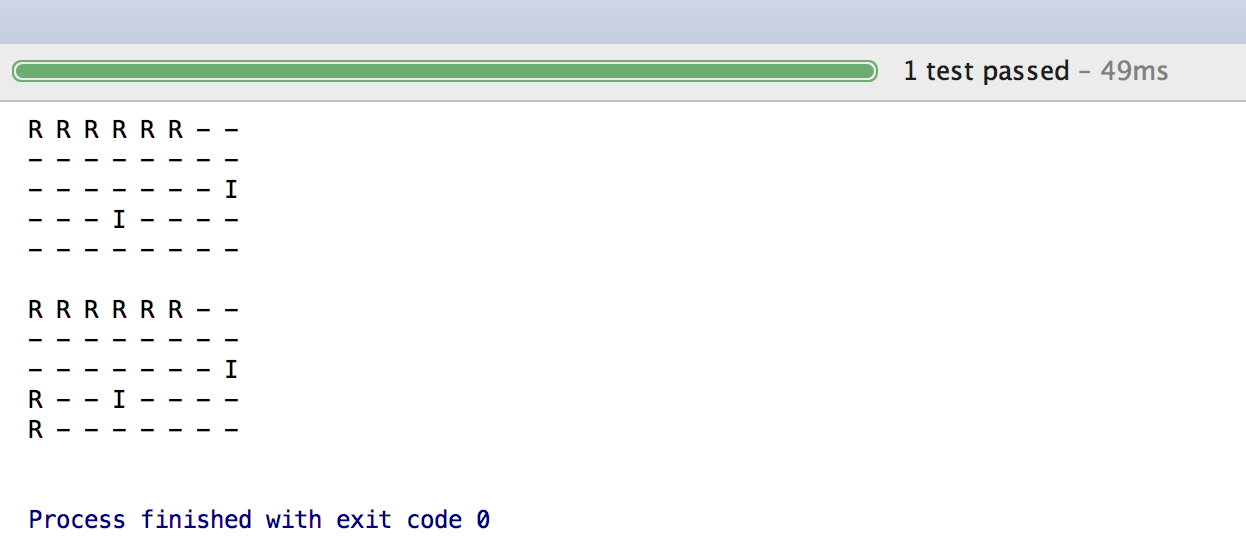
\includegraphics[scale=0.5]{test_mapgrid}}

\section{Roads}\label{roadsection}
\subsection{Basic Structure}
\paragraph{}
A road is defined as a container for one or more lanes with a start point and an end point of type Coordinate. This allows us to track the position of the road and consequently add an Intersection or not to the end of the road. Each road is connected to at most two intersections. Our roads can be of size 1 to n and only can be drawn horizontally or vertically according to the start and end point locations. Our simulation system has limited the number of lanes of a road to 2 with a left-hand driving traffic pattern with a maximum length of 30, due to map dimension constraints. If we do not assign an intersection to the end of the road, the vehicle will leave the simulation after reaching the end.
\subsection{Lanes}
\paragraph{}
A lane is part of a road where the vehicles actually move. A lane's length is defined by the road it is part of. The number of cells that vehicles can be in is equal to the length of the lane. Vehicles enter the lanes at the start position and exit through the end position. Lanes are like queues that follow the cellular automata model, i.e. it is first-in-first-out and vehicles can only move forwards if the cell in front of them is empty. 
\paragraph{}
Lanes have a moving direction associated with them by the MapDirection enumeration, which consists of values NORTH, SOUTH, EAST, and WEST. We set this explicitly because if a lane has a length of 1, its start and end locations are the same, therefore making it impossible to determine which way traffic would need to flow. When adding lanes to a road, the lanes travelling north must be added before the ones travelling south and the lanes travelling east must be added before the ones travelling west to maintain the left-hand style of driving.
\paragraph{}
To create a lane we must consider 4 aspects regarding the cardinality:
\begin{itemize}
\item If the map direction is North, then the lane\textsc{\char13}s start point is the road\textsc{\char13}s start point and the lane\textsc{\char13}s end point is the road\textsc{\char13}s end point.
\item If the map direction is South, then the lane\textsc{\char13}s start point is the road\textsc{\char13}s end point and the lane\textsc{\char13}s end point is the road\textsc{\char13}s start point.
\item If the map direction is East,  then the lane\textsc{\char13}s start point is the road\textsc{\char13}s start point and the lane\textsc{\char13}s end point is the road\textsc{\char13}s end point.
\item If the map direction is West,  then the lane\textsc{\char13}s start point is the road\textsc{\char13}s end point and the lane\textsc{\char13}s end point is the road\textsc{\char13}s start point.
\end{itemize}

\subsection{Evaluation}
\paragraph{}
We believe are roads are well implemented. They fulfill their task of holding a number of lanes without any excess overhead. However, a few possible improvements could be possible, such defining a better way of keeping track which lanes are moving in what direction. In other words, lane orientation in the map is defined only by the order in which lanes are added to the road. So if the requirement is to have left-hand side driving, then the north-moving lane must be added before the south-moving lane. Removing this kind of dependency could make it easier adding lanes to roads. Also, our system was only tested with roads with up to two lanes, so including support for more lanes would be possible.

\section{Traffic Lights}\label{trafficlights}
\subsection{Basic Structure}
\paragraph{}
The TrafficLight class is a fairly simple class that implements traffic light functionality for the simulation. Each traffic light has a duration (how long it should last a single colour) and initial state (red or green). It subscribes to the Ticker upon creation. The nextState() method takes the state it is currently in and sets it to the state it should be in next.

\subsection{Ticker Interaction}
\paragraph{}
This is where most of the interesting implementation lies. Each traffic light holds an internal time. On each ticker tick, if its internal time is less than the duration, it increments its internal time. If it hits its duration, it changes to the next colour and resets its internal time. To tell the rest of the system of its colour change, it tells the traffic light controller of its new colour state.

\subsection{Traffic Light Controller and Traffic Light Decorator}
\paragraph{}
The TrafficLightController class is the link between the model TrafficLight class and the GUI representation. It follows the singleton pattern, and includes global variables like the duration of all traffic lights and whether or not the traffic lights are enabled. It also includes two "database" type objects: a HashMap, with each TrafficLight instance registering to its GUI representation, and an ArrayList that holds all TrafficLight instances.
\paragraph{}
The "colourChanged(LightColour colour, TrafficLight tl)" method gets called by the traffic light "tl" with the new "colour" it is. This method then takes the traffic light "tl" and uses it as a key to look up its corresponding GUI representation, a TrafficLightDecorator, in the HashTable. Each TrafficLightDecorator contains a TrafficLight that it is representing and a JavaFX Circle shape. The circle is what actually changes the colour upon request. First the circle is drawn, and when the "setGUIColour(LightColour colour)", the circle changes colour to the new colour.
\paragraph{}
The TrafficLight controller also contains helper methods as well as support for disabling and enabling all traffic Lights and changing the duration of all traffic lights.

\subsection{Evaluation}
\paragraph{}
We believe that using a HashTable to store (TrafficLight, TrafficLightDecorator) pairs in the controller was a good idea because of its O(1) retrieval time. At first, we were unsure of how to have many intances of TrafficLights linked to TrafficLightDecorators. We first considered having many instances of the controller, but that did not make logical sense, as the controller should be able to control all TrafficLights from one instance. Having the HashMap made it easier to look up which circles must change colour at any given time. However, a minor change that could be possible is removing the ArrayList of TrafficLight instances and only using the HashMap keys to get at a list of all traffic lights. This would remove a data redundancy.

\section{Intersections}\label{intersectionsection}
\subsection{Basic Structure}
\paragraph{}
An intersection is a special type of component that connects roads together. It connects at least two roads and a maximum of four. To represent the connections, the intersection has four variables, one for each road. Road positioning relative to that intersection instance is specified by the names of the variables. For example, a road that is north of the intersection gets set as the intersection's north road.
\paragraph{}
An intersection also contains up to four traffic lights. Traffic lights can be determined automatically by the method "setDefaultTrafficLightsForRoads()", which looks at each road that is set to the intersection and sees if there is a lane in that road that is driving towards the intersection. If there is such a lane, then the traffic light is added. To prevent all the traffic lights from starting with the same initial colour, north and south traffic lights start red, and west and east traffic lights start green, but only if there is a traffic light in the north or south slot. If there are no north or south lights, then the east and west traffic lights start at red. For more information about the traffic lights in the intersection, look at Section \ref{trafficlights} on page \pageref{trafficlights}.
\subsection{Intersection Controller and Decorator}
\paragraph{}
The intersections have a controller to act as a link between their model and view representations. A HashMap is used in the controller to keep a sort of "database" where each intersection is registered with exactly one instance of an intersection GUI representation.
\paragraph{}
Each IntersectionDecorator class is associated with a single intersection instance. Each has up to 4 TrafficLightDecorators that live inside this GUI. The Intersection does not have any explicit circles itself, it relies on the circles of each TrafficLightDecorator that is associated with each TrafficLight in the Intersection instance. Exactly one IntersectionDecorator is created for exactly one Intersection.
\paragraph{}
The most important functionality of the Intersection decorator is the drawIntersection method that draws the wrapped Intersection and produces a visual representation with traffic lights embodied in a stack pane:
\begin{lstlisting}
	public StackPane drawIntersection() {
		...
		return stackPane;	
	}
\end{lstlisting}
The locations for each traffic light are determined. Then, for each traffic light, if it is not null, its circle representation gets added to the interection GUI representation.
\subsection{Evaluation}
We believe that our intersections are well designed. At first, we were unsure of how to display up to four traffic lights at once. By embedding TrafficLightDecorators inside the IntersectionDecorator we were able to display all traffic light circles at once. There was an issue that we had to solve which involved only one of the circles changing colour, despite them all being visible and set to the correct initial states. This was solved by including a method in the TrafficLightDecorator class to return the circle to the IntersectionDecorator and have it manage the drawing and adding the actual circle to the view. This may have been a simple issue with JavaFX panes, because it was always the last added traffic light that would change colour. However, this way, there is a controller that manages combining a few traffic lights into one grid cell view. 

\section{Ticker}
\paragraph{}
The ticker class is how time is kept in the simulation system. It would start at zero and increment at a given time increment, or granularity, such as every one second. Any type of object that wants to do some operation at every time increment must subscribe to this class. The ticker publishes the time to all subscribers at every time increment. Typical subscribers include vehicles and traffic lights, although other objects can subscribe as well.
\paragraph{}
The Ticker class is located high up in the package hierarchy because of how central its role is. It was one of the tricker parts of the project implementation because we had to decide how to implement the publish-subscribe relationship and have the ticker ticking at a constant rate. The ticker had to once be re-worked because of some complexity that arose. However, the one aspect that remained constant was the importance of having the publish-subscribe relationship.
\subsection{First Implementation}
\subsubsection{Initial Stages}
\paragraph{}
In the first implementation of the Ticker class, important things had to be decided on, such as how to notify all subscribers of time changes and how to handle time ticking on a periodic basis. Because we were starting from scratch, we had nothing to base it on, so the design was one of the more difficult parts of the implementation.
\subsubsection{Basic Structure}
\paragraph{}
The Ticker class followed the singleton pattern, so that the number of instances would be capped at one. The constructor was marked with the protected visibility so that only the class itself would be able to call the constructor (as well as any subclasses, but there are none). Any potential subscribers would implement an interface called TickerListener, which contained a method called "onTick(long time)" that needed to be implemented by the subscriber. This would be the method that would execute on every time increment in the ticker.
\subsubsection{Ticking Support}
\paragraph{}
The actual underlying ticking relied on two main aspects: a Timer instance and a TimerTask instance (both part of the java.util package). In general, a Timer instance executes a TimerTask instance at the specified interval. The Ticker class had a class embedded in it, called TickerRunnable which extended the TimerTask class. It also followed a singleton pattern for the constructor and it had a "run()" method that would execute when required by the Timer. This is where each subscriber would be notified with the current time in the simulation. To start the Ticker ticking, it had a method called "start()", which initiated the Timer and gave it the task of running the TickerRunnable at the given interval specified by the variable of type long named TICK\_INTERVAL. So overall, after every interval, the TickerRunnable would execute its "run()" method, which would tell all subscribers that the time changed, which would execute some operation. For instance, vehicles would move forwards.
\subsubsection{Evaluation}
\paragraph{}
The Ticker class performed well with the model elements of the project. In the test cases performed, vehicles would move properly and traffic lights would change colour. However, there were many issues that had to be resolved. Firstly, we did not like the way in which subscribers were notified of time ticks. The Ticker held a list of all its subscribers, which already violates the key property of the publish-subscribe relationship (publishers of events do not know who its subscribers are, nor should they care). Because of this list, on every tick, we would cycle through this list and notify each subscriber one at a time. This was not ideal because some subscribers would hear the tick before others. This made us think of how we could try to notify all subscribers at once.
\paragraph{}
Secondly, and more importantly, this implementation did not work with JavaFX threads. An exception would be thrown each time a thread other than the JavaFX thread would try to modify any graphical elements. This was first discovered when we tried to test the GUI representation of traffic lights. We would get the following exception:
\begin{lstlisting}
	Exception in thread "Timer-1" java.lang.IllegalStateException:
	Not on FX application thread; currentThread = Timer-1
\end{lstlisting}
This was a major cause for concern, because the goal was to have a fully functioning graphical user interface and not simply displaying vehicles in the console! At first, this was solved by a call to the JavaFX application platform, called Platform. It contains a method "runLater(Runnable r)" that takes any sort of runnable task. This did make the animation work from the Ticker thread, but it was not ideal because it simply schedules the task for some "unspecified time in the future". Finally, a minor issue was that the Ticker had an instance, but all methods were static, so it made us think if having an instance was necessary at all. This is when we decided that the Ticker class must be re-worked in some other way, hence our second, and current, implementation.
\subsection{Second Implementation (Current)}
\subsubsection{Initial Stages}
\paragraph{}
Given the issues faced with the first implementation, we needed a Ticker that would work with the JavaFX thread and that would ideally notify all subscribers at the same time of the tick. We decided to research potential ways the Ticker could be implemented.
\subsubsection{Getting Help from Libraries}
\paragraph{ReactFX}
This is a library that helps by adding support for "reactive event streams" that works with JavaFX. In short, it processes events that happen in the system, such as clicks \cite{reactfx}. As the first solution, we used a type of event stream called "EventStreams.ticks(...)", which generated a tick after each time the given time  interval passes. This worked for small cases and test files using JavaFX, but due to lack of good documentation, we were unsure of how to proceed with this framework to support the whole simulation system. This library claimed to be inspired by RxJava, a more general reactive approach, so we investigated this next.
\paragraph{RxJava}
Made by ReactiveX and Netflix, this open-source library provides a reactive programming approach for Java \cite{rxjava}. By the word "reactive", it means that there are some objects that react to something else, which means that many reactions can execute in parallel. There are observers (which are subscribers) that listen to some Observable (the publisher). The observable emits some sort of object and the subscribers react to it when they get the message \cite{reactivex}. We decided to use this library as part of our implementation. Although this library can do many other things with  event streams, like filtering or debouncing, we are only skimming the surface of its functionality and only using its publish-subscribe facilitation.
\paragraph{RxJavaFX}
Also made by ReactiveX, this is a library that allows an asynchronous reactive approach to JavaFX-specific events. It is useful for GUI event processing \cite{rxjavafx}. Although we decided to use this in our Ticker implementation, we are using a very small amount of its functionality. The only aspect of this library that we are using is specifying that the publisher/observable should run on the JavaFX application thread.

\subsubsection{Solution}
\paragraph{}
We decided to use a combination of RxJava and RxJavaFX for our Ticker implementation. The thing that does the actual ticking is defined as an Observable$<$Long$>$ from the RxJava package, rx. The type parameterization says that the message that this publisher sends is of type Long. This is so the current time in the system can be sent. Objects that wish to subscribe to the Ticker must extend the Subscriber$<$Long$>$ class, also from the rx package. This gives the subscriber three methods to implement: onCompleted(), which gets called once the Ticker terminates, onError(Throwable t), which gets called if there is an error with the Ticker, and most importantly, onNext(Long long), which gets called on every tick. Classes like Vehicle and TrafficLight implement this method to define functionality that must be performed on every tick. To subscribe to the observable's messages, each subscriber class is set to call Ticker.subscribe(...) in its constructor with itself as the parameter. This executes the following line for each subscriber:
\begin{lstlisting}[language=Java,breaklines=true,basicstyle=\small]
     tickerObservable.takeUntil(stop).observeOn(JavaFxScheduler.getInstance()).subscribe(sub);
\end{lstlisting}
This tells the observable/publisher to subscribe the subscriber "sub" (a vehicle, traffic light, or anything else), to run it on the JavaFX thread, and to make it run until a stop signal is sent to it (it can still unsubscribe sooner than the signal). The resulting behaviour is that when there is a subscriber for the observable, the Ticker starts and the subscribers perform their onNext operations when a tick is sent out.

\subsubsection{Evaluation}
\paragraph{}
This approach works very well with the JavaFX thread because of explicitly specifying ".observeOn(JavaFxScheduler.getInstance())", thanks to RxJavaFx. It is simple to add more subscribers and have them perform some operation, thanks to RxJava. There are only a few downsides with this approach. First, the ticker speed must be set before the simulation begins. Once there is a subscriber, the ticker speed cannot change. For this reason, we request the user sets the ticker speed before beginning the simulation. It is possible in theory, but due to time constraints, we left it as-is. This, in turn, requires calling Ticker.start() once the ticker speed is set to initialize the observable in-charge of ticking. Second, whatever class that wants to subscribe to the ticker must extend the Subscriber$<$Long$>$ class. Therefore, this would be the only class that the subscriber would be able to extend, as Java does not support multiple inheritance.
\paragraph{}
Also made by ReactiveX, this is a library that allows an asynchronous reactive approach to JavaFX-specific events. It is useful for GUI event processing. Although we decided to use this in our Ticker implementation, we are using a very small amount of its functionality. The only aspect of this library that we are using is specifying that the publisher/observable should run on the JavaFX application thread.

\section{Vehicles}
\paragraph{}
The simulation system is, after all, about vehicles and how they behave in different maps and conditions. This section will go in-depth into how vehicles move and the different types that are possible.
\subsection{The Vehicle Class}
\paragraph{}
Vehicle is abstract class that all vehicles implement; it enapsulates all generic vehicle behaviour. It being abstract allows for scalability because we can add more types of vehicles such as cars and ambulances. There are two types of vehicles: cars and ambulances. The Car and Ambulance class extend Vehicle. To describe the vehicle movement in this program, it is important to mention that each lane is an array list of vehicles, and also lanes are queues (First-In-First-Out), so the first vehicle that enters a lane is the first vehicle to leave.   
\paragraph{}
Vehicles have a lot of attributes that are either global for all types of instances or are specific to an implementation. Attributes that define vehicles are: priority, behaviour, location, and state. Vehicle priority is represented by an integer, with 1 being the lowest. Vehicle behaviour is represented by an enumeration called VehicleBehaviour, with possible values of average, aggressive, or cautious. Coordinate location is determined dynamically by the "getCurrentCoordinate()" method. Finally, state is determined dynamically by calling all relevant vehicle movement methods and assigning it based on the outcome, which is based on the current state of the simulation.
\subsubsection{Car}
\paragraph{}
Instances of Cars are the most common in the simulation. This class extends the Vehicle class to gain all vehicle functionality but with some Car specific attributes. Cars represents basic vehicles, with basic vehicle behaviour. Cars are initialized with average behaviour and with the lowest priority of 1.
\subsubsection{Ambulance}
Instances of ambulances represent a vehicle with high priority. It is initialized with aggressive behaviour and a priority of 5, which is the highest in our system so far.
\subsection{Vehicle Movement and Ticker Interaction}
\paragraph{}
All significant vehicle behaviour is because of its interaction with the Ticker. On every tick by the ticker, the vehicle calls the VehicleController to move. The controller finds the corresponding VehicleDecorator, the GUI representation, in a HashMap of (Vehicle, VehicleDecorator) pairs. Then we begin processing the vehicle's request to move in the moveVehicle method.
\paragraph{}
Vehicles movement can be divided into two main categories: moving in a lane and turning to a new lane. Before any movement happens, we set the previous lane and coordinate of the vehicle to it's current lane and coordinate keep track of.
\subsubsection{Moving in a lane}
As we mentioned, each lane is an array of vehicles, so the movement of vehicles is simply changing the vehicle's position in the lane by increasing its index by adding a number of steps. Vehicles only move forwards when the slot in front of it is empty. Cars are type of vehicle with AVERAGE behaviour, and our team decided to make an Average behaviour move vehidles one step each time. On the other hand, vehicles with AGGRESSIVE behaviour such as ambulances, move two steps each time if possible, otherwise one step at a time. To decide if a vehicle can move, there are two conditions: If the new cell is empty, which means no vehicle is already there, or if the new cell is in the lane boundary.
If these conditions are met, the vehicle moves, otherwise it stops.
To move it, we set the current cell to null, so other vehicle can move to this cell and increase the vehicle's index by the number of steps it moved.
\subsubsection{Turning to a new lane}
After controlling the vehicle movement in a lane, we went to manage the movement of vehicle to other lanes. Vehicle can turn to a new lane only throw intersections, which means it has to be at in the end of its current lane. To move to a new lane there are three main things we considered: Reading traffic lights, choosing the next lane to move to, and the ability to turn.
\paragraph{Reading traffic lights}
In our program, each road has two lanes, and each intersection can connect up to four Roads, which means each intersection can have up to four traffic lights. The readTrafficLight() method in the Vehicle class controls that each vehicle reads only its corresponding traffic light. Reading the correct traffic light depends on the map direction of a lane. For example, if the map direction of a lane is south, and the vehicle is at the end of its lane, that means this vehicle is in the north road for this intersection it has to read the north traffic light, and so on for other directions. If the traffic light is red, vehicle state is set to 0, which means vehicle stops, and if it is green, vehicle state sets to 1, which means vehicle can move. Vehicle with higher priority such as ambulances always can move even if the traffic light is red. After making vehicle listen to traffic lights, we moved to choose a new lane to move to.
\paragraph{Choosing the next lane to move to} 
Vehicles can only turn when they are at the end of the current lane. Vehicles reads the intersection in front if it and then read all roads connected to that intersection. From these roads, we take only go to lanes with a legal map direction for a given vehicle. For example, assume vehicle A is in a west road and its driving direction is East, and this vehicle want to move to the south road. As we mentioned, each road has two lanes with different map directions. For the south road, there are two lanes, one with north map direction and the other with south map direction. So, vehicle A can only choose lane which map direction is south. 
"ArrayList$<Lane>$ getLaneOptions()" checks all connected lanes to an intersection and tests the validity of lanes in terms of the map direction and state. If the map direction is legal for a vehicle and the lane state is 1 (lane is enabled), this method put possible lanes in an array list. 
"Lane chooseLane()" takes the array list of all valid lanes and chooses a random lane for the vehicle.
\paragraph{The Ability to Turn}
To avoid vehicle crashes in intersections when they turn, we have to regulate the vehicle movement in intersections, one vehicle at a time. The first idea was to use vehicle IDs. Since each vehicle has a unique ID we can compare them, vehicle with higher ID moves, other wait. After generating large numbers of vehicles on a map, we decided comparing IDss was not a good choice. Assuming there are 50 vehicles on a map (vehicles id will be from 1 to 50) and there are two full lanes of vehicles connected to an intersection, each vehicle in these lanes want to turn. If the vehicle at the front of the queue has an ID of 3, all vehicles behind that vehicle have to wait too. This made us give vehicles priorities to turn. The idea is to give vehicles at intersections a "vehiclePriorityToTurn" value which is a random number from one to four, all unique, in terms of the maximum number of vehicles in an intersection is four. The vehicle with the highest vehiclePriorityToTurn value moves, otherwise it waits.

We first implemented a method to give vehicles vehiclePriorityToTurn values and to compare values to decide who moves first. Vehicle priorities are not like vehicle IDs because each vehicle has a unique and same ID all the time, so no need for setting new IDs each time they are at an intersection. But by using priority, we need to give each vehicle a new priority each time they are at an intersection. When we implemented a method to give vehicles vehiclePriorityToTurn values in the Vehicle class, each vehicle gives other vehicles new priority, in other words, assume we have 4 cars at an intersection C1, C2, C3, and C4: 
\begin{enumerate}\itemsep1pt \parskip0pt \parsep0pt
\item C1 will give it self and others priority
\item C2, will give it self and other priority, witch C1 already did
\item C3, will give it self and other priority, witch C1 and C2 already did
\item C4, will give it self and other priority, witch C1, C2 and C3 already did
\end{enumerate}
Then each vehicle compares it own priorities. So, for example in number 1: C3 is the largest priority and it moves. But in number 2, C1 is the largest priority so it moves too, at the same time with C1. So the problem still remains.

However, what we did next is implement "ArrayList<Vehicle> giveVehiclePriorities (ArrayList<Integer> randomPriority)" in the Intersection class, which makes giving priority comes from intersections, not vehicles, to give each vehicle a unique priority. Therefore, the Intersection became a subscriber of the Ticker, so it can decide on each tick who will turn next. The "giveVehiclePriorities" method has three major jobs:
\begin{enumerate}\itemsep1pt \parskip0pt \parsep0pt
\item Sets vehicles at intersections vehiclePriorityToTurn to a random number from one to four.
\item Sets the corresponding traffic light for each vehicle at intersection.
\item Return an array list of all vehicles at intersection.
\end{enumerate}
The "vehicleTurnFirst (ArrayList<Vehicle> vehicles)" method in the Intersection class takes the array list of vehicles at intersection as a parameter and compare the vehiclePriorityToTurn only for vehicles where their traffic light state is GREEN, then sets the vehiclePriorityToTurn to 1 for the  vehicle with higher vehiclePriorityToTurn, or vehicles with vehiclePriority equal to 5 such as ambulances, otherwise sets to 0 .

The final step to make vehicles turn is in "int vehicleTurn(Lane l)" method in Vehicle class. This method checks four things:
\begin{enumerate}\itemsep1pt \parskip0pt \parsep0pt
\item If a vehicle is at the end of its lane.
\item If the chosen lane is not null.
\item If the first cell in the chosen lane is empty.
\item If vehiclePriorityToTurn equals to 1.
\end{enumerate}
If these conditions are obtained, vehicle turns, otherwise stops.
To sum up, vehicles read traffic light, if it is red vehicles stop except ambulances which can move. If traffic light is green, vehicles choose random available lanes and check their abilities to move. Vehicles which obtained the conditions move otherwise, stop.

\paragraph{}
Note that all movement methods, such as turning or moving straight, return an integer, which we call "move". It is like a boolean, except with more information about the result. If move gets set to zero, that means the vehicle did not move and therefore we should not animate the vehicle movement. If move is greater than one, then the vehicle can be animated to move. However, if move was set to three, that means the vehicle should be removed from the simulation. All the movement methods may or may not actually move the vehicle in the model. When we go to do the vehicle animation, this is where the previous lane and coordinate come in. We must now animate the vehicle from its previous lane and coordinates, not its new ones, otherwise the vehicle would be moved twice. 

\subsection{Evaluation}
Making the Vehicle class an abstract class was a good idea because this makes our system extensible to new types of vehicles in the future. Fixing the vehicle movement bugs, namely when two vehicles would drive into the same lane at the same time, was a large accomplishment due to its real-time complexity. In terms of general vehicle movement, an area for improvement could be the steps taken to move. Maybe there is a better way of doing the animation, instead of setting the previous lane and coordinates and doing the animation based on that. But other than that, we believe that the Vehicle class performs very well regarding the different states a vehicle can hold and the different movement results that can be returned. Therefore, vehicles are robust to any kind of map or driving conditions.

However, vehicles do not know, if there is an ambulance behind them. In future work, we would vehicles cleverer in their movement, so if there is an ambulance behind them they should have the higher vehiclePriorityToTurn, so ambulance can move faster.  Vehicles do not step on each other in intersection, they always follow their priority to turn. It would be better if more than one vehicle can move at the same time if their paths do not clash.
If there are no traffic lights in an intersection, vehicles turns depending on their priority to turn, so they never crash in intersections.

Vehicles can choose any valid lane connected to their intersection. So, they always have a list of all available lane options and they can choose a random lane only form the list. Vehicles never go to a wrong lane. However, making U-turn is not allowed yet in the system.

\section{Log}
\paragraph{}
The simulation system writes a log file with the corresponding timestamp each time the simulation starts. The log file name is with the form "Log\_Year-Month-Day-Hour-Minute-Second" and it gets stored in the "logs" directory in the working directory, i.e. where the source code is or where the executable is placed. Each object that is subscribed to the ticker is appended to the log with all its attributes. We are able to trace on each tick the activity generated by the object and it is useful for debugging processes, audits, and statistics.
\paragraph{}
To achieve the logging functionality we use the java.util.logging.Logger and we also extend the log class to the subscriber so it can interact easily with the Ticker to write the state of every subscriber on each tick.

\section{Testing the System}
\paragraph{}
Before we had our GUI screens, we tested the logic of our system using JUnit testing. In the src directory, we have a "test" package. This is where all of our test files went. We used JUnit tags such as @assertEquals(...), @assertNotNull(...), @Before(), and more. This allowed us to see whether the outputs we were expecting were achieved. 
\paragraph{}
However, tests involving the Ticker were done using main() methods, because we found that JUnit did not support multiple threads in its text environment. We researched into this some more, but found it easiest to use the main() methods in our test cases for our testing purposes. Additionally, once we had some GUI screens, we relied less on JUnit testing and more on integration testing using those screens.

\part{The Application}
\section{Start-Up}
\paragraph{}
When the user starts the system, they get presented with a start screen. After pressing the start button, the user gets presented with a choice of modes: opening a map or creating a new map. The screens are loaded using a series of controllers. A singleton instance of the StartUpController is made, which controls the first few screens.
\paragraph{}
Opening a map opens a File dialog where the user can open a pre-made map file. The simulation comes with some map files pre-built for the user. This then brings the user to the simulation screen. The StartUpController hands control over to the SimulationController, which handles drawing the SimulationScreen. 
\paragraph{}
Choosing to make a map brings the user to the Map Maker screen. They choose a width and height of a map, place components on it, and save it as a new map. The user can then run the simulation on it. The StartUpController hands control over to the MapMakerController, which handles drawing the MapMakerScreen.
\paragraph{}
Here is a use-case diagram that describes the steps the user can take in our system:
\paragraph{}
\centerline{ 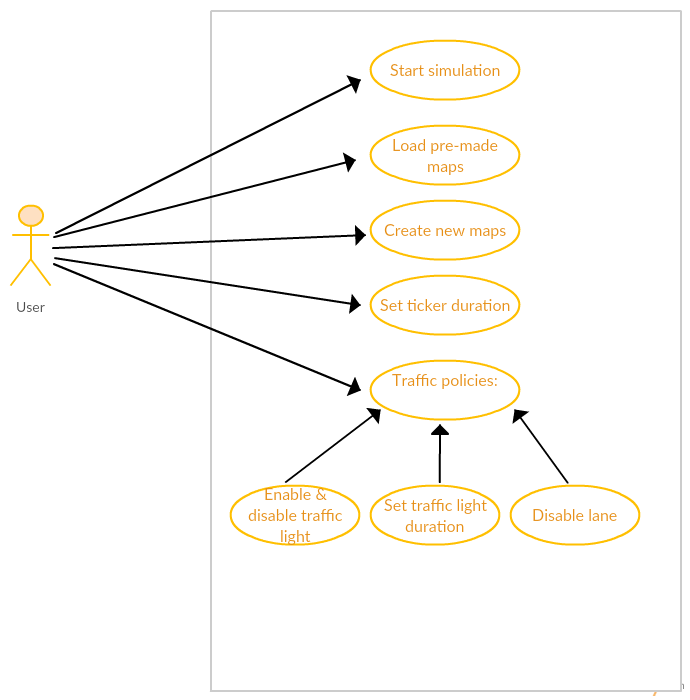
\includegraphics[scale=0.5]{UseCase}}

\section{Simulation Screen}
\paragraph{}
Aimed at making a user-oriented simulation system, we decided to have a main simulation screen where users can both monitor the simulation process and control the simulation system by using various controls. Users would load maps from file to run the simulation on.
\subsection{Loading Maps}

\subsection{Overall Screen Structure}
\subsubsection{JavaFX Scene Builder}
\paragraph{}
Concerned that JavaFX Scene Builder is a visual layout tool that lets users to quickly design JavaFX application user interfaces, without coding but can just drag and drop UI component to a work area, modify their properties, apply style sheets, and the FXML code which is automatically generated in the background can be combined with a Java project by binding the UI to the application's logic to handle the events and actions taken on each element, we chose JavaFX Scene Builder as our main user interfaces development tool at first.
\paragraph{}
Problems arose after we finished building FXML file and  tried to connect the UI interface with simulation models. We found only one controller can be used in a FXML file which means we need to figure out how to communicate between different controllers. This problem first arose when we loaded pre-made map into the simulation. 
\paragraph{}
Users need to choose a pre-made map before going into simulation screen, this will need an intermediate controller to deliver map name between two interfaces. There will be lots of this kind of communication so that lots of intermediate controllers need to be added which will increase complexity potentially. Thinking about this, we finally gave up JavaFX Scene Builder, decided to use pure JavaFX.

\subsubsection{Simulation Screen}
\paragraph{}
The simulation screen Interface was built using Model-View-Controller (MVC) architecture pattern. SimulationController.java is the controller to draw the screen and generate the log for the simulation. SimulationScreen.java is the corresponding model used to manage UI components of the interface. 
\paragraph{}
We used the built-in layout container classes, called panes that are available with the JavaFX SDK to manage UI components of simulation screen. The JavaFX SDK provides several layout panes for the easy setup and management of classic layouts such as rows, columns, stacks, titles, and others. As a window is resized, the layout pane automatically repositions and resizes the nodes that it contains according to the properties of the nodes. We used BorderPane layout pane for the simulation screen. The BorderPane layout pane provides five regions in which to place nodes: top, bottom, left, right and center. 
\paragraph{}
To keep the interface simple and clear, only three parts were used in our simulation screen: top, center and right. Title of the simulation screen "LondonSW Simulation System" was set on the top of the BorderPane . We used the center part to load the chosen pre-made map in which simulation process will happen. The right part was mainly used to monitor and control the simulation process. Here we used the VBox layout pane to make sure nodes are arranged in a single column. 
\paragraph{}
Labels including "Number of Cars", "Ticker interval", "Traffic Light Duration", "Time Ticked", "Vehicle Time Spent Standing" were set for simulation monitor to help users have a better understand about how is the simulation process going. 
\paragraph{}
"Start" and "Reset" buttons are used to control whether to start or stop the simulation process. Users can click "Add Ambulance" to add an ambulance whose behavior is aggressive and can also delete it since once an ambulance is added the button will be "Delete Ambulance". There is a "Set Traffic Light duration" button. Once it is clicked, there will be a dialog allows users to set traffic interval(100-1000 millisecond) by a spinner. "Disable Traffic Light" is used to delete all traffic lights of the map and "Enable Traffic Light" to restore all traffic lights to the map. This is to simulate situation in which traffic lights cannot work properly. 
\paragraph{}
We used a slider to control number of cars in the system. Users can set number of cars they want as long as  it is in the available range. The minimum car number is 1, the maximum number is set automatically depends on the overall number of slots of all lanes in the map ($MaxCarNumber=0.6*SlotsNumber$). This means the simulation process won't crash due to too many cars results in no slot is available and to make sure the traffic can be coordinated properly. 
\paragraph{}
In JavaFX a property is more than just a simple value. Each Property provides methods to observe changes made to its value so that we can listen for changes.The valueProperty of the slider can indicate if the slider is in the process of being changed. And it is an observable property, so we registered a change listener to the slider's valueProperty to know when the slider's value is changing. Slider.valueProperty() gives us access to the Property. AddListener(...) expects a ChangeListener of type Number. We created a new class to implement the ChangListener interface. Since we will use this class only once, it's a bit overkill to create an instance of this class and pass it to addListener(...). Instead we used a short form of creating a class and instantiating it which is actually an anonymous inner class that does not have a name. Every time a change occurs, ChangeListener must have a changed(...) method that will be called. Then we decided whether to generate new cars to the system or remove cars from the system by calculating the difference between the oldValue and the newValue of the slider.
If oldValue is smaller than newValue, new cars $(newValue - oldVlue)$ would be generated to the map. Otherwise, system would delete $(oldValue - newValue)$ cars randomly from the vehicle list. 

\subsection{Map Graphics}
\paragraph{}
For the map creation we are using a suite of Panes which are included in the JavaFX Software Platform. We use stacked panes which allow us to treat different panes like layers and that grants us major management. The whole grid layout consists on a GridPane which is a flexible grid of rows and columns that holds in each row and column a specific pane. Each pane is a box which can either be grass (empty square), a Road, or an Intersection. All are drawings are of our own authorship because we have used the tool GIMP, an open source graphic editor. The size of each stack pane is dynamic and we are able to change it by changing a resize factor, which is an important attribute used in many of our drawings. 
\subsection{Decorators}
\paragraph{}
Our implementation is using the Decorator Pattern to extend the functionalities of each component so that the objects can be drawn by wrapping the original object and invoking a draw method for each component. There are 5 main wrappers MapGridGUIDecorator, IntersectionDecorator, RoadGUIDecorator, TrafficLightDecorator and VehicleGUIDecorator.
\subsubsection{MapGridGUIDecorator}
\paragraph{}
This is the class that manages the drawing of the entire map. By traversing the MapGrid representing the Map, we check what type of component is in each cell. We call the corresponding decorator class for that type of component. 
\subsubsection{RoadGUIDecorator}
\paragraph{}
The Road is a stack pane that has a rough grey background and the arrows of the lane representing which way traffic flows are drawn programatically in each square.
\subsubsection{IntersectionDecorator}
\paragraph{}
The intersection is drawn with the same background as a Road but in addition it has a yellow diagonal cross. For information about drawing intersections, please refer to section \ref{intersectionsection} on page \pageref{intersectionsection}.
\subsubsection{TrafficLightDecorator}
\paragraph{}
The traffic lights are also drawn programatically using its decorator class. For information about drawing traffic lights, please refer to section \ref{trafficlights} on page \pageref{trafficlights}.
\subsubsection{VehicleGUIDecorator}
Vehicle movement is displayed by using the VehicleGUIDecorator class. 
Each vehicle will have exactly one VehicleGUIDecorator associated with it. We have defined different states of the vehicle so we can track their movements and make them move properly:
\begin{itemize}\itemsep1pt \parskip0pt \parsep0pt
\item State 0 is when a vehicle is not moving
\item State 1 means that the vehicle is moving straight.
\item State 2 means that the vehicle has entered an intersection
\item State 3 is a state where the vehicle has been deleted or has exited the simulation.
\end{itemize} 

\subsection{Evolution of Vehicle Drawing and Animation}
\paragraph{}
Our vehicle movement evolved over the course of the project, with many improvements made along the way. 
\subsubsection{First Implementation}
\paragraph{}
After the map's grid was able to be drawn dynamically, the vehicle now had to move on top of the lanes. It was challenging at first because the obvious way of having the vehicle move between grid cells is not possible. The first step towards our solution was having a rectangle representing the vehicle fill the whole grid cell, regardless of whether it is moving vertically or horizontally. The location of where the rectangle should go was determined by a formula, which took its original placement in the map. The coordinate x- and y-positions of the vehicle are multiplied by the image dimension and the resize factor. The actual movement of the vehicle was dependent on the map direction it is coming from and the map direction it is going to. So if a vehicle is moving east, then north, that means it is turning left and a left turn animation was required. A JavaFX TranslateTransition is used to move the vehicle.
\paragraph{}
However, turning the vehicle was quite complex. In the first implementation, a vehicle would simply shift into its new location, so a different edge of the vehicle would now be moving forwards. That did not lend itself to a realistic simulation. Additionaly, because of all the different kinds of cases of movement, like east to north, west to south, et cetera, had a lot of duplicated code with only a few values changed in each. Furthermore, the nature of the animation was shifting it by some x and y values relative to where the vehicle currently is. This made the animation imprecise and over time, vehicles would shift out of their lanes and start moving on grass or on top of other improper lanes. As a consequence, this kind of animation did not work with any ticker speed. If the ticker was made faster, the animation would become more imprecise, with vehicles not reaching the cells they should have in time. This approach worked well in a very limited amount of cases and needed to be reworked to work with a variety of ticker speeds and many vehicles. This brought us to our second implementation of vehicle movement.

\subsubsection{Second Implementation (Current)}
\paragraph{}
Because of all the issues with the first vehicle movement, namely vehicles shifting out of place and not working with various ticker speeds, we re-worked the animation to a much simpler process. The process is:
\begin{enumerate}\itemsep1pt \parskip0pt \parsep0pt
\item Get the current coordinate location of the vehicle
\item Calculate the new coordinate location for the vehicle
\item Calculate the required vehicle rotation based on where it is moving from and to
\item Determine the actual pixel locations for the new location
\item Set the movement translation to an exact location
\item Move and rotate the vehicle
\end{enumerate}
There are helper methods to calculate some of the steps. The method "directionToTranslation(MapDirection d)" takes a MapDirection and translates it into a coordinate representing a movement in that direction. For example, passing in a parameter of EAST returns a Coordinate with the value of (1,0), which represents moving once in the positive x-direction and staying constant in the y-direction. The method "getRotationFromDirectionChange(...)" takes the direction the vehicle is moving from and to as parameters and returns the angle which the vehicle must turn by. Most importantly, the method "coordinateToPixels(Coordinate c, MapDirection d)" takes a location in the map and a direction as parameters and returns the exact location to where the vehicle must move to. It is also used to determine the initial location of the vehicle. The MapDirection parameter makes sure that the vehicle gets drawn in the correct lane.

\paragraph{}
There are many advantages to this second implementation. First, there was a drastic reduction in code duplication. The process was converted to a set of simple steps, like a recipe, which works in any situation. In addition, because of each coordinate having a distinct location, the vehicle knows exactly where to move to. This makes it work flawlessly with any ticker speed. Finally, the vehicle does not shift out of its proper lane over time. 

\subsection{Simulation Statistics}
We have a couple of traffic management policies. These are:
\begin{itemize}\itemsep1pt \parskip0pt \parsep0pt
\item Changing the duration of traffic lights
\item Disabling or enabling traffic lights
\item Increasing or decreasing the number of vehicles
\end{itemize}
\paragraph{}
By doing these three things, the effect of them can be seen in the "Vehicle Time Spent Standing" statistic. This is a percentage that gets calculated using all the vehicles in the map. Each vehicle has two variables associated with it for the calculation of this statistic: timeSpentStanding and timesTicked. Each time the vehicle was unable to move, its timeSpentStanding increases. A vehicle is unable to move if it is at a red light or if there was a vehicle in the slot in front of it. The increment happens VehicleController class when the "move" result is zero, i.e., it could not move forwards.
\begin{lstlisting}
	if(move == 0) {
		Vehicle thisVehicle = vehicleGUIDecorator.getVehicle();
		thisVehicle.incrementTimeSpentStanding();
	}
\end{lstlisting}
\paragraph{}
For the percentage calculation, there is a local subscriber to the ticker in the SimulationScreen class. It is used for doing anything operation when the ticker ticks, like increasing the "Times Ticked" label and doing this statistic calculation. Each time the ticker ticks, the method "getPercentageStanding()" is called and the output is set to the label.
\paragraph{}
In this function, the VehicleController gets queried for two values: the total time spent standing for all vehicles and the total times ticked for all vehicles. Each method gives the sum of all timeSpentStanding and timesTicked, respectively. 
\begin{lstlisting}
	int timeSpentStanding = VehicleController.getTotalTimeSpentStanding();
	int totalTimesTicked = VehicleController.getTotalTimesTicked();
\end{lstlisting}
\paragraph{}
To get the average time spent standing statistic, the following calculation is made:
\begin{lstlisting}
	double ans = (double) timeSpentStanding / totalTimesTicked * 100;
	return Math.round(ans * 100.0) / 100.0;
\end{lstlisting}
\paragraph{}
This statistic can tell us about the amount of congestion on the roads and how external factors like traffic lights can affect vehicle movement over time.

\subsubsection{Interesting Trends}
\paragraph{}
Many interesting reactions to this statistic can be observed by manipulating the three controls available: increasing and decreasing the number of vehicles, disabling traffic lights, and setting the traffic light duration.
\begin{itemize}
\item The more vehicles there are, the higher the percentage of vehicle time spent standing is.
\item When holding the simulation conditions stable (e.g. keeping a constant number of vehicles, not changing traffic light duration), the percentage of vehicle time spent standing stabilizes over time and does not differ by about one percentage.
\item Increasing the duration of traffic lights increases the percentage of vehicles standing, and decreasing the duration of traffic lights decreases the percentage of vehicle time spent standing.
\item Disabling traffic lights does not completely bring the percentage of vehicle time spent standing to zero. This is because there may still be other vehicles getting in the way.
\item Setting the number of vehicles to zero resets the statistic because every car in the simulation is new.
\item Adding one more vehicle to the simulation does not affect the statistic significantly.
\end{itemize}

\section{Map Maker Mode}
\subsection{Map Making Basics}
\paragraph{}
To make our system more flexible to different kinds of maps, we allow the user to build their own maps to run the simulation on if they do not like any of the pre-made maps. When starting the system, if the user chooses to "Make a new Map", they are prompted to choose a width and height. To prevent maps that are too small or large to view, the width and height are limited to the range of 5 to 30. An empty map of the width and height that they chose is generated. The user can then proceed to put map components into the grid by clicking on the desired component and clicking to where on the map they want the component to be. Map components include: intersections, roads that run vertically (North-South), roads that run horizontally (East-West), and grass (an empty, or null, square). Roads are always added with a lane going in each direction. If a component was placed in a square by accident, the "grass" component can be added to empty that map grid square. The user keeps doing this until the map they build is complete. At that point, the user would press the "Save Map" button to save the map to disk. If the user does not like their map, the "Reset Map" button removes all components from the map. If they decide to not build a map anymore, the "Go Back" button brings them back to the mode selection screen. 

\subsection{Implementation}
\paragraph{The Empty Map}
The empty map is represented by the Map class, which contains the MapGrid of no components. To allow clicking on the map, we traverse through the map, visiting each cell, and adding an on-click listener to each cell. Since the Map is represented by a JavaFX GridPane, getting the node to add the on-click listener to at the specified location was not trivial. We included a function called "getNodeFromIndex" that takes the x- and y-coordinates and the GridPane as parameters. It gets the node by looking throught all the children of that GridPane cell for every GridPane cell, and if that Node's location equals the location that we requested, that Node from the GridPane is returned. Now we know when the user clicks on the map to place a map component.
\paragraph{Placement of Map Components}
When the user selects a component from the right of the screen and clicks on a location in the map, an instance of that component is actually created in the map. For instance, when placing an intersection in the map, an Intersection object gets created and placed in that space. It is set with no roads attached and no traffic lights. When placing a bit of road, either North-South or East-West, an instance of the Road class is created every time. The Road instance's start and end coordinate locations are the same, so a road of length 1 is created. Two lanes are added, with each going in opposite directions.
\paragraph{Keeping Focus}
At first, building maps was a very annoying task. The user would have to click on the map component on the right, then click on the empty grid square, then go back to click on the map component again, followed by an empty grid square, and so on. This was solved by tracking of what on the screen gets focus and what held the focus previously. Focus means what was last clicked or selected  by the user, that is, the mouse cursor was "focused" on a specific element on the screen. The focus is represented by a Java enum, with entries like ROADNS (for a road that travels vertically) and INTERSECTION. 
\paragraph{}
When this mode starts up, the current focus is set to nothing, and the previous is null. The values are stored in the MapMakerController. As an example, if the user first clicks on the Intersection component image, that image gains focus. A blue glow surrounds the image to represent that it has focus. If the user then clicks on an empty map grid square, that map grid square gains focus and the previous focused gets set to Intersection. The map grid checks was was previously focused. It will see that Intersection ws previously focused, and place the component in the clicked map grid square. However, to make it easier on the user, focus is then placed back on the Intersection component image so they can keep clicking intersections into the map. The same applies for all other component images. 
\paragraph{Saving the Map}
When the user decides to save the map, they first get prompted for a file name. The file name cannot be empty, and this is enforced by disabling the "OK" button in the Save dialog while the name text field is empty. When the user hits the "OK" button, the saving process begins. Because of the way the map components were placed into the map, all the roads are separate and disconnected and all intersections are not connected to any roads. In other words, if there is a road of length 5 moving vertically, there are actually 5 separate roads moving vertically. We need to "glue" together all the bits of roads, connect those roads to the relevant intersections, and add all traffic lights. 
\paragraph{}
There is a method in the MapMakerScreen class called "buildAndSaveMap(Map m)" that takes the map "m" that the user built. Using that map's width and height, the method creates a new empty map that will serve as the "glued together" and final verison of the user built map. We traverse the broken map, and when we discover a component, we process it. Discovering an intersection is the simplest case. We remove the intersection from the old map and place a new intersection into the old map at the same location. For bits of Road instances, it is trickier. If we discover a bit of road that is moving horizontally (east-west), we then have a while loop moving down the map row to see how long the road is. This way we determine the start location of this road (the original found piece) and the end location of this road (the last bit of road discovered moving horizontally that was not null). We create a new road, add 2 lanes, remove all the bits of road from the old map (so they do not get added again to the fixed map), and add the new road to the new map. A similar process is done for roads moving vertically. Each time a new stretch of road bits is discovered in the old map, this process is followed to "glue" all road sections together.
\paragraph{}
Now that we added all Roads and Intersections to the new map, we must connect the "edges" and "nodes" of our map, i.e. our roads and intersections. There is a method called "assignRoadsToIntersections(Map m)" that takes the fixed map that we just built as a parameter. We retrieve the list of all intersections from the map, and determine the surrounding coordinates for that intersection. If there is a road component in any of the coordinates, the intersection gets assigned that road. For example, if there is a Road component at the location one coordinate north of the intersection, that road gets assigned as the north road of that intersection. This is done for all intersections. Now that all roads are glued and all intersections have been assigned roads, the map can now finally be saved to disk.
\paragraph{}
We are using Java serialization to save the map. First, we check if the maps directory exists. The maps directory is set to the current working location from where the system was invoked. If it does not exist, it is created. Using the file name that the user provided in the Save dialog, we save it into the maps directory. Once this is complete, the user gets taken to the previous screen in the system, the choose mode screen. Now they can choose to open their newly built map or build a new one.
\paragraph{Map Validation and Robustness}
When saving the map, there is no map validation. We do not check whether all roads connect to some intersection and that no intersections are floating alone with no roads. Therefore, the user is able to build any meaningless or broken maps. However, this is completely fine. The simulation is robust against these kinds of map designs by having the vehicles behave in appropriate ways. For instance, if there is a road without an intersection at the end of it, the vehicle simply leaves the simulation. If there is a road connected to an intersection, but no other roads to go to, the vehicle simply stays in place once it reaches the intersection because it has nowhere else to go. So overall, no matter how poorly built the map is, the vehicles will act accordingly and there will be no system crashes.

\subsection{Evaluation}
Although the map building process was optimized by keeping focus and quick map component placement, there are a few areas where the process could have been improved. Some sort of click-and-drag functionality would make it easier to place a lot of components in big maps. Some of the non-GUI functionality, like saving the map or helper methods like getting a Node at some coordinate, could have been moved to the controller to keep GUI and logical methods separate. When saving the map, we should have probably checked if each newly discovered adjacent bit of road is moving in the same direction as the first piece of discovered road. Some map validation would be nice to have, regardless of how robust the system is. Finally, a dialog saying where the map was saved to would be useful so the user would know exactly where to look when trying to load their map for the simulation screen.

\part{Teamwork}
\section{Communication}
\paragraph{}
We use WhatsApp for general communication, like coordinating meeting times. We use Slack for project discussion, like discussing new ideas/problems and sharing documents. We have general discussion for all group members and private communication between two members to talk about issues like program interfaces without bothering others.

\section{Group meetings}
\paragraph{}
We have scheduled group meetings twice a week, mostly on Monday and Friday. We discussed task progress and assigned new tasks normally on Monday. On Friday, there would be a long-duration meeting. we would talk about the project in detail and members would code together.
\section{Agile development with Mingle}
\paragraph{}
Because of the nature of the project, continuous learning and adaptation to the emergent state of the project are unavoidable. We use Mingle for project management which is based on Agile software development principles. It is designed to integrate with a team's current workflow. We used Mingle's Planner feature to define objectives for each team members, track a plan's progress, and receive alerts when a plan changes. Mingle helps our team communicate and collaborate easily and effectively solve problems by having more efficient conversations with team members.
\paragraph{}
At the task level, Mingle allows us to assign teammates to a specific action, so everyone can see who is working on what. At each end of our group meeting we will assign tasks to group members by adding a new story at Mingle planner including a specific task description, an estimate duration, status (new, in progress, complete), a task priority (must, should could), the owner of the task. 
\paragraph{}
At the project level, we use Mingle to nudge teams to have a conversation if an upcoming deadline has not been met. Before each group meeting we will talked about task completion status to have a better grasp about how is the progress going.
\paragraph{}
At the program level, Mingle sends us alerts so that everyone can follow up. we also exported the task file and uploaded to Github to make it available and more convenient  for everyone to check their tasks at any time.
 
\subsection{Github}
\paragraph{}
IntelliJ is our main platform for coding. We use Github as our main source-code repository. We have a master branch and four personal branches. Everyone is free to experiment and commit changes. Anything in the master branch is always deployable. Branch won't be merged until it's ready to be reviewed by master. Once we have done our tasks we may make a commit so that others can follow to understand after pulling. We would add an associated commit message, which is a description explaining why a particular change was made to make it clear for others what we have done. Master branch would close a merge and we could also rolled  back changes if a bug found since each commit is considered a separate unit of change.

\part{General Project Evaluation}
\section{Things that went well}
\paragraph{}
We had clear goals for each development stage, i.e. what must/should/could be achieved for each iteration. Before and after each iteration, we would check and make sure everything has been achieved. This ensures our entire development process is progressing well. By following Agile development principles, our team did a good job responding to unpredictability through incremental and iterative work. 
\paragraph{}
From the perspective of software development, we adhered to the MVC architecture. We have clear hierarchical model structures, e.g., a map contains roads and intersections, traffic light and lane are owned by intersection and road respectively.
\paragraph{}
We made the system an user-friendly application. Users can monitor and control the simulation process by going into simulation mode. The map maker mode allows users to design maps with any dimensions or map components. A simulation log is available after each simulation for users to analyze the whole simulation process. 
\paragraph{}
In general, we worked well as a team, with each member focusing on a different aspect of the system. There were no major conflicts and everyone understood the importance of good, hard work for this project.

\subsection{Things that did not go well and what we did}
We had many difficulties along the way, but we always managed to pull through and resolve them. The ticker went through several iterations itself, with improvements being made each time. The animation started off basic, which also got improved several times over the course of the project. Bugs like traffic lights not working in loaded maps got fixed promptly. And finally, the resize factor used to display maps poorly, but now does a good job for all map sizes.

\subsection{Possibilities for the future}
\paragraph{}
It is impossible to implement all ideas we had because of short term. In the future, we can add more vehicle types like police cars, bicycles, buses, etc. as well as more road types including railroads and overpasses. There can be arc intersections instead of cross intersections. We can make our system adapt to real maps like Google Maps. By providing a real location, users can get traffic situations through our system. By connecting background log files to real maps, it would be possible to deliver these log files to real traffic monitoring stations for furthter-step traffic analysis.

\part{Peer Assessment}
\paragraph{}
We have decided to distribute the points as follows:

\part{Appendix}
\section{Git Log}
\begin{center}
\begin{longtabu} to \textwidth {|
    X[4,l]|
    X[3,c]|
    X[8,l]|}
    \hline
    \textbf{Author} & \textbf{Date} & \textbf{Message} \\ \hline
violetavk & 2016-01-22 & Initial commit \\ \hline
Violet & 2016-02-08 & initial structure created \\ \hline
Violet & 2016-02-08 & added some more classes for importing maps (from OpenStreetMap) \\ \hline
Violet & 2016-02-08 & Moved project files and added .gitignore \\ \hline
Violet & 2016-02-08 & First report draft \\ \hline
Violet & 2016-02-08 & Second draft \\ \hline
Violet & 2016-02-08 & Merging in `reports' \\ \hline
Violet & 2016-02-08 & Third draft of initial report \\ \hline
Violet & 2016-02-09 & Final version of initial report \\ \hline
Violet & 2016-02-10 & Adding comments for all the classes we have so far as to what they should do \\ \hline
yakubu & 2016-02-10 & added coordinate class \\ \hline
rawanmoh & 2016-02-10 & updates car class \\ \hline
Jia & 2016-02-10 & This is the Class of Intersection \\ \hline
jia0627 & 2016-02-10 & This is the Class of Intersection \\ \hline
jia0627 & 2016-02-10 & AnimationTimer \\ \hline
santiago & 2016-02-11 & Demo Version \\ \hline
santiago & 2016-02-11 & Merge remote-tracking branch `origin/master' \\ \hline
rawanmoh & 2016-02-11 & update car class \\ \hline
rawanmoh & 2016-02-11 & update car class \\ \hline
rawanmoh & 2016-02-11 & update car class \\ \hline
violetavk & 2016-02-11 & added some code to Lane and Road; added equals method to Coordinate; added JUnit test for Lane \\ \hline
rawanmoh & 2016-02-12 & update car class \\ \hline
Violet & 2016-02-12 & Forgot to add libraries for junit tests yesterday; added potential controller for View; added another method to Lane; started RoadTest class \\ \hline
felix & 2016-02-12 & Added test for coordinates and changed exception in lane \\ \hline
felix & 2016-02-12 & Updates to intersection \\ \hline
rawanmoh & 2016-02-12 & update car class \\ \hline
rawanmoh & 2016-02-12 & Merge remote-tracking branch `origin/master' \\ \hline
rawanmoh & 2016-02-12 & update car class \\ \hline
Violet & 2016-02-12 & Adding CarDirection, MapDirection, LaneTest update \\ \hline
rawanmoh & 2016-02-12 & update car class \\ \hline
yakubu & 2016-02-12 & Traffic Lights \\ \hline
Violet & 2016-02-12 & Updates to Lane \\ \hline
yakubu & 2016-02-12 & LaneTest \\ \hline
yakubu & 2016-02-12 & Merge remote-tracking branch `origin/master' \\ \hline
Violet & 2016-02-12 & adding trafficlighttest \\ \hline
yakubu & 2016-02-12 & LaneTest \\ \hline
yakubu & 2016-02-12 & changing git ignore \\ \hline
yakubu & 2016-02-12 & Merge remote-tracking branch `origin/master' \\ \hline
yakubu & 2016-02-12 & Traffic light test \\ \hline
santiago.anda@outlook.com & 2016-02-13 & Change variable names \\ \hline
santiago.anda@outlook.com & 2016-02-13 & Change variable names \\ \hline
felix & 2016-02-13 & Map and TickerInterval changes \\ \hline
jia & 2016-02-15 & Intersection validation check \\ \hline
Violet & 2016-02-15 & Updates to Lane arguments and MapDirection \\ \hline
Violet & 2016-02-16 & Adding some basic GUI screens \\ \hline
rawanmoh & 2016-02-16 & Add choose vehicle direction randomly \\ \hline
rawanmoh & 2016-02-16 & Merge remote-tracking branch `origin/master' \\ \hline
4ND4 & 2016-02-16 & Update README.md \\ \hline
violetavk & 2016-02-16 & Merge pull request \#1 from 4ND4/master \\ \hline
rawanmoh & 2016-02-17 & create vehicle Test modify Vehicle class \\ \hline
Violet & 2016-02-17 & Updates to Road class \\ \hline
Violet & 2016-02-17 & Merge branch `master' of https://github.com/violetavk/LondonSW\_trafficsimulator \\ \hline
Violet & 2016-02-17 & uncommented Alert dialog in StartUpController \\ \hline
rawanmoh & 2016-02-17 & Merge remote-tracking branch `origin/master' \\ \hline
Violet & 2016-02-17 & Merge branch `master' of https://github.com/violetavk/LondonSW\_trafficsimulator \\ \hline
yakubu & 2016-02-17 & test \\ \hline
jia & 2016-02-17 & intersection test \\ \hline
rawanmoh & 2016-02-17 & pull reauest test \\ \hline
violetavk & 2016-02-17 & Merge pull request \#4 from mugu101/master \\ \hline
violetavk & 2016-02-17 & Merge pull request \#3 from RawanMoh/master \\ \hline
violetavk & 2016-02-17 & Merge pull request \#2 from Jia0627/master \\ \hline
Violet & 2016-02-17 & Adding Ticker class functionality \\ \hline
Violet & 2016-02-17 & Adding Map and Simulation updates \\ \hline
Violet & 2016-02-17 & Updating readme a little \\ \hline
Violet & 2016-02-17 & Adding a grid system to our map \\ \hline
Violet & 2016-02-17 & forgot to add grid integration \\ \hline
Violet & 2016-02-17 & test file into view \\ \hline
yakubu & 2016-02-17 & traffic light states \\ \hline
violetavk & 2016-02-17 & Merge pull request \#5 from mugu101/master \\ \hline
jia0627 & 2016-02-17 & progress report \\ \hline
jia0627 & 2016-02-17 & Merge branch `master' of https://github.com/violetavk/LondonSW\_trafficsimulator \\ \hline
violetavk & 2016-02-17 & Merge pull request \#6 from Jia0627/master \\ \hline
jia & 2016-02-17 & Intersection validation check when setting a new road getRoadOptions \\ \hline
violetavk & 2016-02-17 & Merge pull request \#7 from Jia0627/master \\ \hline
Violet & 2016-02-18 & Changes to MapGrid, Map, and Road \\ \hline
rawanmoh & 2016-02-18 & remove: vehicleLifTime vehicleDirection and their methods \\ \hline
rawanmoh & 2016-02-18 & remove: vehicleLifTime vehicleDirection and their methods \\ \hline
rawanmoh & 2016-02-18 & remove: vehicleLifTime vehicleDirection and their methods \\ \hline
violetavk & 2016-02-18 & Merge pull request \#8 from RawanMoh/master \\ \hline
Violet & 2016-02-18 & Adding ticker \\ \hline
rawanmoh & 2016-02-19 & remove some carDirection method \\ \hline
violetavk & 2016-02-19 & Merge pull request \#9 from RawanMoh/master \\ \hline
rawanmoh & 2016-02-19 & Add vehicle Behavior \\ \hline
jia0627 & 2016-02-19 & intersection validation change \\ \hline
jia0627 & 2016-02-19 & Merge branch `master' of https://github.com/violetavk/LondonSW\_trafficsimulator \\ \hline
violetavk & 2016-02-19 & Merge pull request \#10 from RawanMoh/master \\ \hline
rawanmoh & 2016-02-19 & //new \\ \hline
rawanmoh & 2016-02-19 & //new \\ \hline
jia0627 & 2016-02-19 & intersection validation change \\ \hline
jia0627 & 2016-02-19 & Merge branch `master' of https://github.com/violetavk/LondonSW\_trafficsimulator \\ \hline
violetavk & 2016-02-19 & Merge pull request \#11 from Jia0627/master \\ \hline
Violet & 2016-02-19 & added misc.xml to gitignore \\ \hline
Violet & 2016-02-19 & Merge branch `master' of https://github.com/violetavk/LondonSW\_trafficsimulator \\ \hline
yakubu & 2016-02-19 & New traffic Light Class \\ \hline
violetavk & 2016-02-19 & Merge pull request \#12 from mugu101/master \\ \hline
Violet & 2016-02-19 & update to gitignore \\ \hline
rawanmoh & 2016-02-19 & Add moveVehicle and its test \\ \hline
rawanmoh & 2016-02-19 & Add moveVehicle and its test \\ \hline
violetavk & 2016-02-19 & Merge pull request \#13 from RawanMoh/master \\ \hline
felix & 2016-02-19 & Add class MapTest \\ \hline
violetavk & 2016-02-19 & Merge pull request \#14 from 4ND4/master \\ \hline
felix & 2016-02-19 & Validation corrections \\ \hline
felix & 2016-02-19 & Added more tests to Intersection class \\ \hline
violetavk & 2016-02-19 & Merge pull request \#15 from 4ND4/master \\ \hline
Violet & 2016-02-19 & Integrated Ticker with Traffic light; run TrafficLightTest main method to see how it works \\ \hline
felix & 2016-02-20 & Update test \\ \hline
4ND4 & 2016-02-20 & Add class MapTest \\ \hline
felix & 2016-02-20 & Add class MapTest \\ \hline
4ND4 & 2016-02-20 & Add class MapTest \\ \hline
4ND4 & 2016-02-20 & Add class MapTest \\ \hline
4ND4 & 2016-02-20 & Add class MapGridGUI \\ \hline
felix & 2016-02-20 & Add class MapGridGUI \\ \hline
violetavk & 2016-02-20 & Merge pull request \#16 from 4ND4/master \\ \hline
yakubu & 2016-02-21 & Some tiny tweaks to traffic light and an animation to show switching of the lights \\ \hline
violetavk & 2016-02-21 & Merge pull request \#17 from mugu101/master \\ \hline
4ND4 & 2016-02-21 & Add class MapGridGUI \\ \hline
4ND4 & 2016-02-21 & Resource folder \\ \hline
4ND4 & 2016-02-21 & MapGridGUITestMain \\ \hline
violetavk & 2016-02-21 & Merge pull request \#18 from 4ND4/master \\ \hline
4ND4 & 2016-02-21 & CarGUI Implementation \\ \hline
violetavk & 2016-02-21 & Merge pull request \#19 from 4ND4/master \\ \hline
rawanmoh & 2016-02-21 & read trafficLight \\ \hline
rawanmoh & 2016-02-22 & readTrafficLight test \\ \hline
Violet & 2016-02-22 & Made Ticker class a singleton class, use Ticker.getInstance() to get the ticker \\ \hline
jia0627 & 2016-02-22 & Report2 \\ \hline
rawanmoh & 2016-02-22 & Add moveVehicle and its test \\ \hline
rawanmoh & 2016-02-22 & TODO \\ \hline
violetavk & 2016-02-22 & Merge pull request \#20 from Jia0627/master \\ \hline
violetavk & 2016-02-22 & Merge pull request \#21 from RawanMoh/master \\ \hline
yakubu & 2016-02-22 & Debug colour change \\ \hline
violetavk & 2016-02-22 & Merge pull request \#22 from mugu101/master \\ \hline
Violet & 2016-02-22 & Fixed some moveCar bugs in Vehicle, car didn't move thru the lane before \\ \hline
Violet & 2016-02-22 & Adding the beginnings of ticker integration with car, still some strange behaviour left over \\ \hline
Violet & 2016-02-22 & Fixed traffic light blink problems \\ \hline
Violet & 2016-02-22 & Fixed some Ticker related bugs for Vehicle, working slightly better now \\ \hline
jia0627 & 2016-02-22 & Progress Report3 \\ \hline
jia0627 & 2016-02-22 & getLaneOptions for Intersection \\ \hline
violetavk & 2016-02-22 & Merge pull request \#23 from Jia0627/master \\ \hline
rawanmoh & 2016-02-22 & Add vehicleTurn, it turns and does not choose same lane but still there are some problems \\ \hline
rawanmoh & 2016-02-22 & try commit \\ \hline
rawanmoh & 2016-02-23 & getLaneOptions \\ \hline
Violet & 2016-02-23 & Merge branch `RawanMoh-master' \\ \hline
Violet & 2016-02-23 & merge of Intersection class \\ \hline
Violet & 2016-02-23 & Integrated Ticker with Vehicle fully (hopefully) \\ \hline
Violet & 2016-02-23 & Fixed bug in MapGrid when adding intersection and fixed bug in Intersection addEastRoad \\ \hline
Violet & 2016-02-23 & Added Map serialization, Maps can now save and load \\ \hline
rawanmoh & 2016-02-23 & getLaneOption is complete. \\ \hline
Violet Avkhukova & 2016-02-23 & Merge pull request \#25 from RawanMoh/master \\ \hline
rawanmoh & 2016-02-23 & getLaneOption Test. \\ \hline
rawanmoh & 2016-02-23 & needs to modify getRoad and getIntersection methods \\ \hline
rawanmoh & 2016-02-23 & added lane.setIntersection and its test \\ \hline
yakubu & 2016-02-23 & seperation of functionality: ran into some problems \\ \hline
rawanmoh & 2016-02-24 & modify getLaneOptions and added its test also tests for lane.getIntersection, intersection.getRoad and vehicleTurn \\ \hline
Violet Avkhukova & 2016-02-24 & Merge pull request \#26 from RawanMoh/master \\ \hline
Jia & 2016-02-24 & simulationModeScreen \\ \hline
jia0627 & 2016-02-24 & Merge branch `master' of https://github.com/violetavk/LondonSW\_trafficsimulator \\ \hline
Violet Avkhukova & 2016-02-24 & Merge pull request \#27 from Jia0627/master \\ \hline
4ND4 & 2016-02-24 & Map Dimension changeable Added a resize Factor Programmatically draw roads according to amount of lanes \\ \hline
Violet Avkhukova & 2016-02-24 & Merge pull request \#28 from 4ND4/master \\ \hline
jia0627 & 2016-02-24 & Report4 \\ \hline
Violet Avkhukova & 2016-02-24 & Merge pull request \#29 from Jia0627/master \\ \hline
rawanmoh & 2016-02-24 & Add ROAD as parameter in Lane \\ \hline
Violet Avkhukova & 2016-02-24 & Merge pull request \#30 from RawanMoh/master \\ \hline
yakubu & 2016-02-24 & Separated test functionality from gui logic. created new light but controller isn't able to simultaneously control both.Think it has something to do with threads. \\ \hline
yakubu & 2016-02-24 & Merge branch `master' of https://github.com/violetavk/LondonSW\_trafficsimulator \\ \hline
Violet Avkhukova & 2016-02-24 & Merge pull request \#31 from mugu101/master \\ \hline
4ND4 & 2016-02-24 & Car working properly on road \\ \hline
Violet Avkhukova & 2016-02-25 & Merge pull request \#32 from 4ND4/master \\ \hline
Violet & 2016-02-26 & Added getComponent method to Map \\ \hline
felix & 2016-02-26 & CarGUI Implementation \\ \hline
4ND4 & 2016-02-26 & MapGrid Improvements \\ \hline
Violet Avkhukova & 2016-02-26 & Merge pull request \#33 from 4ND4/master \\ \hline
4ND4 & 2016-02-26 & FixedMap hc serial \\ \hline
Violet Avkhukova & 2016-02-26 & Merge pull request \#34 from 4ND4/master \\ \hline
4ND4 & 2016-02-26 & Map serial change \\ \hline
Violet Avkhukova & 2016-02-26 & Merge pull request \#35 from 4ND4/master \\ \hline
Jia & 2016-02-26 & map creation \\ \hline
Violet Avkhukova & 2016-02-26 & Merge pull request \#36 from Jia0627/master \\ \hline
Jia & 2016-02-26 & report 5 \\ \hline
4ND4 & 2016-02-26 & latest changes \\ \hline
Violet Avkhukova & 2016-02-26 & Merge pull request \#37 from Jia0627/master \\ \hline
Violet Avkhukova & 2016-02-26 & Merge pull request \#38 from 4ND4/master \\ \hline
4ND4 & 2016-02-28 & Map Improvements \\ \hline
Violet Avkhukova & 2016-02-28 & Merge pull request \#39 from 4ND4/master \\ \hline
yakubu & 2016-02-28 & Getting current coordinate improvements and tests \\ \hline
Violet Avkhukova & 2016-02-28 & Merge pull request \#40 from mugu101/master \\ \hline
4ND4 & 2016-02-29 & Fixed map movement \\ \hline
4ND4 & 2016-02-29 & Fixed map movement \\ \hline
felix & 2016-02-29 & Fixed map movement \\ \hline
felix & 2016-02-29 & Fixed map movement \\ \hline
felix & 2016-02-29 & Fixed map movement \\ \hline
felix & 2016-02-29 & Merge branch `master' of https://github.com/violetavk/LondonSW\_trafficsimulator \\ \hline
felix & 2016-03-01 & Merge branch `master' of https://github.com/violetavk/LondonSW\_trafficsimulator \\ \hline
felix & 2016-03-01 & Merge branch `master' of https://github.com/violetavk/LondonSW\_trafficsimulator \\ \hline
felix & 2016-03-01 & Merge branch `master' of https://github.com/violetavk/LondonSW\_trafficsimulator \\ \hline
rawanmoh & 2016-03-01 & coordinate \\ \hline
4ND4 & 2016-03-01 & Car now draws on the corresponding lane \\ \hline
4ND4 & 2016-03-01 & Car now draws on the corresponding lane \\ \hline
rawanmoh & 2016-03-01 & some tests getLaneOptions turnVi \\ \hline
rawanmoh & 2016-03-01 & some tests getLaneOptions turnVi \\ \hline
rawanmoh & 2016-03-02 & some tests getLaneOptions turnVi \\ \hline
Violet Avkhukova & 2016-03-02 & Merge pull request \#41 from RawanMoh/master \\ \hline
felix & 2016-03-02 & Car now draws on the corresponding lane \\ \hline
felix & 2016-03-02 & Merge branch `master' of https://github.com/violetavk/LondonSW\_trafficsimulator \\ \hline
4ND4 & 2016-03-02 & Added RoadIndex \\ \hline
Violet Avkhukova & 2016-03-02 & Merge pull request \#42 from 4ND4/master \\ \hline
Violet & 2016-03-02 & Adding Intersection Decorator things and bug fix in Ticker \\ \hline
Violet & 2016-03-02 & updates to trafficlightcontroller \\ \hline
Violet & 2016-03-02 & fixed a bug in Intersection class \\ \hline
Violet & 2016-03-02 & updates to intersection controller \\ \hline
Violet & 2016-03-02 & Merge branch `master' of https://github.com/violetavk/LondonSW\_trafficsimulator \\ \hline
rawanmoh & 2016-03-02 & some tests getLaneOptions turnVi \\ \hline
Violet & 2016-03-02 & merged changes \\ \hline
felix & 2016-03-02 & Added RoadIndex \\ \hline
Violet Avkhukova & 2016-03-02 & Merge pull request \#44 from 4ND4/master \\ \hline
Violet & 2016-03-02 & Added serialVersionUID to all serializable classes \\ \hline
Violet & 2016-03-02 & Updated fixed map, and fixed bug in Intersection setEastRoad \\ \hline
jia & 2016-03-02 & report 6 \\ \hline
rawanmoh & 2016-03-02 & remove Road from Lane constructor \\ \hline
Violet Avkhukova & 2016-03-02 & Merge pull request \#45 from Jia0627/master \\ \hline
Violet Avkhukova & 2016-03-02 & Merge pull request \#46 from RawanMoh/master \\ \hline
Violet & 2016-03-02 & Fixed serialization issue, hopefully maps load across machines now \\ \hline
rawanmoh & 2016-03-02 & set intersection for lanes \\ \hline
Violet Avkhukova & 2016-03-02 & Merge pull request \#47 from RawanMoh/master \\ \hline
yakubu & 2016-03-02 & Rotate Method and Test \\ \hline
felix & 2016-03-02 & Fixed car GUI \\ \hline
rawanmoh & 2016-03-02 & change set intersection for north and west lane to be compatible with MapGridGUI \\ \hline
Violet Avkhukova & 2016-03-02 & Merge pull request \#48 from mugu101/master \\ \hline
4ND4 & 2016-03-02 & Added TODO \\ \hline
jia & 2016-03-02 & SetMapDimension \\ \hline
felix & 2016-03-02 & Added RoadIndex \\ \hline
felix & 2016-03-02 & Added RoadIndex \\ \hline
Violet & 2016-03-02 & Merge branch `RawanMoh-master' \\ \hline
Violet Avkhukova & 2016-03-02 & Merge pull request \#50 from Jia0627/master \\ \hline
Violet & 2016-03-02 & Merge branch `master' of https://github.com/4ND4/LondonSW\_trafficsimulator into 4ND4-master \\ \hline
Violet & 2016-03-02 & Merge branch `4ND4-master' \\ \hline
Violet & 2016-03-02 & refactored trafficlightgui to decorator \\ \hline
Violet Avkhukova & 2016-03-02 & Merge pull request \#52 from violetavk/traffic-light-colours \\ \hline
4ND4 & 2016-03-03 & Added bigger map \\ \hline
Violet Avkhukova & 2016-03-03 & Merge pull request \#53 from 4ND4/master \\ \hline
4ND4 & 2016-03-03 & Changed car colour \\ \hline
4ND4 & 2016-03-03 & Added lane status \\ \hline
felix & 2016-03-03 & Merge branch `master' of https://github.com/violetavk/LondonSW\_trafficsimulator \\ \hline
Violet Avkhukova & 2016-03-03 & Merge pull request \#54 from 4ND4/master \\ \hline
felix & 2016-03-03 & test \\ \hline
4ND4 & 2016-03-03 & added an example test.java of the car turning \\ \hline
jia0627 & 2016-03-03 & SetMapDimension \\ \hline
Violet Avkhukova & 2016-03-03 & Merge pull request \#55 from Jia0627/master \\ \hline
felix & 2016-03-04 & Merge branch `master' of https://github.com/violetavk/LondonSW\_trafficsimulator \\ \hline
rawanmoh & 2016-03-04 & Added lane state in getLaneOptions \\ \hline
Violet Avkhukova & 2016-03-04 & Merge pull request \#56 from RawanMoh/master \\ \hline
felix & 2016-03-04 & Added Interfase Vehicle \\ \hline
4ND4 & 2016-03-04 & Decorated Vehicle \\ \hline
felix & 2016-03-04 & Merge branch `master' of https://github.com/violetavk/LondonSW\_trafficsimulator \\ \hline
felix & 2016-03-04 & Decorated Vehicle \\ \hline
Violet Avkhukova & 2016-03-04 & Merge pull request \#57 from 4ND4/master \\ \hline
yakubu & 2016-03-04 & Road closed image \\ \hline
4ND4 & 2016-03-04 & Single map implementation \\ \hline
Violet Avkhukova & 2016-03-04 & Merge pull request \#58 from 4ND4/master \\ \hline
yakubu & 2016-03-04 & Merge branch `master' of https://github.com/violetavk/LondonSW\_trafficsimulator \\ \hline
yakubu & 2016-03-04 & Road closed image \\ \hline
Violet Avkhukova & 2016-03-04 & Merge pull request \#59 from mugu101/master \\ \hline
rawanmoh & 2016-03-04 & fix VehicleTurn bug \\ \hline
Violet Avkhukova & 2016-03-04 & Merge pull request \#60 from RawanMoh/master \\ \hline
jia & 2016-03-04 & pre-made map \\ \hline
felix & 2016-03-04 & Single map implementation \\ \hline
yakubu & 2016-03-04 & Random cell method \\ \hline
yakubu & 2016-03-04 & Add step method for coordinates \\ \hline
Violet Avkhukova & 2016-03-04 & Merge pull request \#61 from Jia0627/master \\ \hline
Violet Avkhukova & 2016-03-04 & Merge pull request \#62 from 4ND4/master \\ \hline
Violet Avkhukova & 2016-03-04 & Merge pull request \#63 from mugu101/master \\ \hline
Violet & 2016-03-04 & Removed commented code from Intersection \\ \hline
Violet & 2016-03-04 & Adding RxJava and RxJavaFx libraries \\ \hline
Violet & 2016-03-04 & Added new Ticker refactor \\ \hline
Violet & 2016-03-05 & Integrated TrafficLight and Intersection with new Ticker, and fully functioning GUIs for each \\ \hline
Violet & 2016-03-05 & Vehicle fully integrated with new Ticker \\ \hline
Violet Avkhukova & 2016-03-05 & Merge pull request \#64 from violetavk/ticker-refactor \\ \hline
4ND4 & 2016-03-05 & Rules for intersection movement (using transition animation) \\ \hline
felix & 2016-03-05 & Rules for intersection movement (using transition animation) \\ \hline
felix & 2016-03-05 & Rules for intersection movement (using transition animation) \\ \hline
felix & 2016-03-05 & Merge branch `master' of https://github.com/violetavk/LondonSW\_trafficsimulator \\ \hline
Violet Avkhukova & 2016-03-05 & Merge pull request \#65 from 4ND4/master \\ \hline
rawanmoh & 2016-03-06 & Added map \\ \hline
rawanmoh & 2016-03-06 & Merge branch `master' of https://github.com/violetavk/LondonSW\_trafficsimulator \\ \hline
Violet Avkhukova & 2016-03-06 & Merge pull request \#66 from RawanMoh/master \\ \hline
felix & 2016-03-07 & Merge branch `master' of https://github.com/violetavk/LondonSW\_trafficsimulator \\ \hline
Violet Avkhukova & 2016-03-07 & Merge pull request \#67 from 4ND4/master \\ \hline
jia0627 & 2016-03-07 & Report 7 \\ \hline
Violet Avkhukova & 2016-03-07 & Merge pull request \#68 from Jia0627/master \\ \hline
rawanmoh & 2016-03-07 & fix vehicleTurn, If there is no lane to go, the vehicle stops \\ \hline
Violet & 2016-03-07 & Merge branch `RawanMoh-master' \\ \hline
Violet & 2016-03-07 & merge with rawan laneoptions code \\ \hline
Violet & 2016-03-07 & fixed messed up merge for drawTestMapExample, hopefully \\ \hline
rawanmoh & 2016-03-08 & Added JavaDoc to Vehicle Class \\ \hline
Violet Avkhukova & 2016-03-08 & Merge pull request \#70 from RawanMoh/master \\ \hline
Violet & 2016-03-08 & Integrated traffic lights with map, cars do not yet listen to them \\ \hline
Violet Avkhukova & 2016-03-08 & Merge pull request \#71 from violetavk/intersection-integration \\ \hline
Violet & 2016-03-08 & Fixed arrows to show properly and refactored the method, and set test map dimension to 22x22 \\ \hline
rawanmoh & 2016-03-08 & cars listen to traffic light \\ \hline
jia0627 & 2016-03-08 & simulation start\&reset trigger \\ \hline
Violet Avkhukova & 2016-03-08 & Merge pull request \#72 from RawanMoh/master \\ \hline
Violet & 2016-03-08 & Simulation controller added from Jias code \\ \hline
Violet & 2016-03-08 & Merge branch `Jia-master' \\ \hline
Violet & 2016-03-08 & Merge branch `master' of https://github.com/Jia0627/LondonSW\_trafficsimulator into Jia-master \\ \hline
Violet & 2016-03-08 & Merge branch `Jia-master' \\ \hline
Violet & 2016-03-08 & fixed minor bug in readTrafficLight and added some documentation to some methods \\ \hline
yakubu & 2016-03-08 & Coordinate class documentation \\ \hline
Violet Avkhukova & 2016-03-08 & Merge pull request \#74 from mugu101/master \\ \hline
rawanmoh & 2016-03-09 & control the movement of more than car organize MapGridGUITestMain code \\ \hline
Violet Avkhukova & 2016-03-09 & Merge pull request \#75 from RawanMoh/master \\ \hline
rawanmoh & 2016-03-09 & divided drawTestMapExample into one lane and two lane.. \\ \hline
Violet Avkhukova & 2016-03-09 & Merge pull request \#76 from RawanMoh/master \\ \hline
yakubu & 2016-03-09 & Created ambulance which inherits from vehicle \\ \hline
4ND4 & 2016-03-09 & Merge branch `master' of https://github.com/violetavk/LondonSW\_trafficsimulator \\ \hline
Violet Avkhukova & 2016-03-09 & Merge pull request \#77 from mugu101/master \\ \hline
Violet & 2016-03-10 & Deleted CarDecorator and TrafficLightAnimation, added serialization to intersectiondecorator and trafficlightdecorator \\ \hline
Violet & 2016-03-10 & Fixed merge conflicts \\ \hline
rawanmoh & 2016-03-10 & fix a wrong coordinate for road 7 in drawTestMapExample \\ \hline
Violet Avkhukova & 2016-03-10 & Merge pull request \#79 from RawanMoh/master \\ \hline
Violet & 2016-03-10 & WORK IN PROGRESS, some cars moving in the proper lanes \\ \hline
4ND4 & 2016-03-10 & Merge branch `master' of https://github.com/violetavk/LondonSW\_trafficsimulator \\ \hline
felix & 2016-03-10 & Merge branch `master' of https://github.com/violetavk/LondonSW\_trafficsimulator \\ \hline
felix & 2016-03-11 & Merge branch `master' of https://github.com/violetavk/LondonSW\_trafficsimulator \\ \hline
felix & 2016-03-11 & Merge branch `master' of https://github.com/violetavk/LondonSW\_trafficsimulator \\ \hline
felix & 2016-03-11 & Merge branch `master' of https://github.com/violetavk/LondonSW\_trafficsimulator \\ \hline
felix & 2016-03-11 & Merge branch `master' of https://github.com/violetavk/LondonSW\_trafficsimulator \\ \hline
Violet Avkhukova & 2016-03-11 & Merge pull request \#81 from 4ND4/master \\ \hline
Violet & 2016-03-11 & Fixed animation for all cars, it now works with any ticker speed \\ \hline
rawanmoh & 2016-03-11 & generate Vehicle \\ \hline
yakubu & 2016-03-11 & We would have a button to spawn an ambulance:on single and double click \\ \hline
Violet & 2016-03-11 & Merged new animation on top of old code \\ \hline
Violet Avkhukova & 2016-03-11 & Merge pull request \#82 from mugu101/master \\ \hline
Violet & 2016-03-11 & Animation works with multiple cars \\ \hline
Violet & 2016-03-11 & Merge branch `master' of https://github.com/violetavk/LondonSW\_trafficsimulator \\ \hline
Violet & 2016-03-11 & Merged with ambulance code \\ \hline
rawanmoh & 2016-03-11 & Added generateVehicle method \\ \hline
Violet Avkhukova & 2016-03-11 & Merge pull request \#83 from RawanMoh/master \\ \hline
jia0627 & 2016-03-12 & Report8 \\ \hline
Violet Avkhukova & 2016-03-12 & Merge pull request \#84 from Jia0627/master \\ \hline
4ND4 & 2016-03-13 & Merge branch `master' of https://github.com/violetavk/LondonSW\_trafficsimulator \\ \hline
rawanmoh & 2016-03-13 & Added some validation in setCurrentCell and setCurrentLane Added Exceptions in setCurrentCell and setCurrentLane Added some javaDoc in vehicle Class \\ \hline
Violet Avkhukova & 2016-03-13 & Merge pull request \#85 from 4ND4/master \\ \hline
Violet & 2016-03-13 & Trying to fix traffic light serialization \\ \hline
Violet & 2016-03-13 & Merge branch `master' of https://github.com/violetavk/LondonSW\_trafficsimulator \\ \hline
Violet & 2016-03-13 & Fixed merge with rawan's updates \\ \hline
4ND4 & 2016-03-14 & Merge branch `master' of https://github.com/violetavk/LondonSW\_trafficsimulator \\ \hline
Violet Avkhukova & 2016-03-14 & Merge pull request \#87 from 4ND4/master \\ \hline
rawanmoh & 2016-03-15 & change moveVehicle form void to boolean added new test in LaneTest fix move out of intersection bug \\ \hline
Violet & 2016-03-15 & Traffic lights now worked in loaded maps from file \\ \hline
Violet & 2016-03-15 & Added the example map as a file, this one is a complete map \\ \hline
Violet & 2016-03-15 & Merged with fixed move out of intersection \\ \hline
jia0627 & 2016-03-15 & Report9 \\ \hline
rawanmoh & 2016-03-15 & Merge branch `master' of https://github.com/violetavk/LondonSW\_trafficsimulator \\ \hline
rawanmoh & 2016-03-15 & Merge branch `master' of https://github.com/violetavk/LondonSW\_trafficsimulator \\ \hline
rawanmoh & 2016-03-16 & Added car ID \\ \hline
Violet Avkhukova & 2016-03-16 & Merge pull request \#89 from RawanMoh/master \\ \hline
felix & 2016-03-16 & Added some functionalities \\ \hline
Violet & 2016-03-16 & Improved getting the width and size from user for mapmaker mode \\ \hline
felix & 2016-03-16 & Added some functionalities \\ \hline
felix & 2016-03-16 & Added some functionalities \\ \hline
felix & 2016-03-16 & Merge branch `master' of https://github.com/violetavk/LondonSW\_trafficsimulator \\ \hline
4ND4 & 2016-03-16 & Added the click functionality to enable and disable roads \\ \hline
4ND4 & 2016-03-16 & Added the click functionality to enable and disable lanes (clicking on arrow) \\ \hline
felix & 2016-03-16 & Added the click functionality to enable and disable lanes (clicking on arrow) \\ \hline
yakubu & 2016-03-16 & Changes to Ambulance: Works with a single click. Also ambulance behaviour is fine unless we would like to change \ldots{} \\ \hline
Violet Avkhukova & 2016-03-16 & Merge pull request \#90 from 4ND4/master \\ \hline
yakubu & 2016-03-16 & Generating new ambulance on click and removing the old one using rawans car generate method \\ \hline
4ND4 & 2016-03-16 & Cars abandon Simulation when they get to a road without an intersection \\ \hline
yakubu & 2016-03-16 & Able to create new intstances of ambulance. However not able to remove them. Still working on it. \\ \hline
Violet Avkhukova & 2016-03-16 & Merge pull request \#91 from 4ND4/master \\ \hline
Violet Avkhukova & 2016-03-16 & Merge pull request \#92 from mugu101/master \\ \hline
felix & 2016-03-16 & Cars abandon Simulation when they get to a road without an intersection \\ \hline
4ND4 & 2016-03-17 & Cars now disappear properly \\ \hline
Violet Avkhukova & 2016-03-17 & Merge pull request \#93 from 4ND4/master \\ \hline
Violet & 2016-03-17 & Can now add intersections in map maker mode \\ \hline
Violet & 2016-03-17 & Merge branch `master' of https://github.com/violetavk/LondonSW\_trafficsimulator \\ \hline
rawanmoh & 2016-03-17 & Added method in lane to read the vehicle in intersection Added lane as a parameter to moveVehicle \\ \hline
Violet Avkhukova & 2016-03-17 & Merge pull request \#94 from RawanMoh/master \\ \hline
4ND4 & 2016-03-17 & Fix bug when traffic light disabled, and lane disabled car stopped forever \\ \hline
4ND4 & 2016-03-17 & Fixed bug for moveVehicle, now the cars don't go on top of each other when a car stops\ldots{}. \\ \hline
Violet Avkhukova & 2016-03-17 & Merge pull request \#95 from 4ND4/master \\ \hline
rawanmoh & 2016-03-18 & Added method to who turn first \\ \hline
Violet Avkhukova & 2016-03-18 & Merge pull request \#96 from RawanMoh/master \\ \hline
Violet & 2016-03-18 & Added more to Map maker mode \\ \hline
Violet & 2016-03-18 & Merge branch `master' of https://github.com/violetavk/LondonSW\_trafficsimulator \\ \hline
felix & 2016-03-18 & Fixed bug for moveVehicle, now the cars don't go on top of each other when a car stops\ldots{}. \\ \hline
Violet Avkhukova & 2016-03-18 & Merge pull request \#97 from 4ND4/master \\ \hline
jia0627 & 2016-03-18 & Merge branch `master' of https://github.com/violetavk/LondonSW\_trafficsimulator \\ \hline
jia0627 & 2016-03-18 & Merge branch `master' of https://github.com/violetavk/LondonSW\_trafficsimulator \\ \hline
Violet & 2016-03-18 & Added more to MapMaker mode and reworked Simulation mode screens \\ \hline
jia0627 & 2016-03-18 & Merge branch `master' of https://github.com/violetavk/LondonSW\_trafficsimulator \\ \hline
Violet & 2016-03-18 & Adding forgotten SimulationController \\ \hline
yakubu & 2016-03-18 & Done with ambulance class and a few minor changes \\ \hline
Violet Avkhukova & 2016-03-18 & Merge pull request \#98 from mugu101/master \\ \hline
Violet & 2016-03-19 & Can now place new map squares on top of old ones, and fixed a bug in Road runsVertically \\ \hline
Violet & 2016-03-19 & Adding east-west roads and hitting the save button determines which road bits are connected and adds them as one single road \\ \hline
rawanmoh & 2016-03-20 & Added methods to intersection class, do not do any thing yet added map to laneTest \\ \hline
rawanmoh & 2016-03-20 & Added new maptest in mapExample \\ \hline
4ND4 & 2016-03-20 & Added Logs to simulation \\ \hline
Violet Avkhukova & 2016-03-20 & Merge pull request \#99 from RawanMoh/master \\ \hline
Violet Avkhukova & 2016-03-20 & Merge pull request \#100 from 4ND4/master \\ \hline
Violet & 2016-03-20 & Tried something for resize factor \\ \hline
jia0627 & 2016-03-20 & Merge branch `master' of https://github.com/violetavk/LondonSW\_trafficsimulator \\ \hline
Violet & 2016-03-21 & When saving user built map, it can detect which roads should be merged as one \\ \hline
Violet & 2016-03-21 & Added JavaDoc to the MapMaker screen \\ \hline
jia0627 & 2016-03-21 & Merge branch `master' of https://github.com/violetavk/LondonSW\_trafficsimulator \\ \hline
Violet & 2016-03-21 & Added JavaDoc to MapMakerController \\ \hline
jia0627 & 2016-03-21 & update SimulationScreen \\ \hline
Violet & 2016-03-21 & Small additions to MapMakerScreen \\ \hline
Violet & 2016-03-21 & Merge branch `Jia-master' \\ \hline
4ND4 & 2016-03-21 & FIxed issue with car going on top of each other when the cars are not moving \\ \hline
felix & 2016-03-21 & Merge branch `master' of https://github.com/violetavk/LondonSW\_trafficsimulator \\ \hline
felix & 2016-03-21 & FIxed issue with car going on top of each other when the cars are not moving and disappear properly. \\ \hline
jia0627 & 2016-03-21 & report 10 \\ \hline
rawanmoh & 2016-03-21 & new methods \\ \hline
Violet Avkhukova & 2016-03-21 & Merge pull request \#104 from Jia0627/master \\ \hline
Violet & 2016-03-21 & Worked on saving map in map builder, cleaned up some controllers, and deleted unnecessary files \\ \hline
Violet & 2016-03-21 & Deleted useless map, updated BigMap.map so lane disabling works \\ \hline
Violet & 2016-03-21 & Added Back button to MapMaker mode \\ \hline
Violet & 2016-03-21 & Finished map maker mode, can now build a map and run a simulation on it in simulation mode \\ \hline
jia0627 & 2016-03-21 & finish add/delete ambulance \\ \hline
Violet Avkhukova & 2016-03-21 & Merge pull request \#105 from Jia0627/master \\ \hline
Violet & 2016-03-21 & Changed the Log a little to save them in the logs directory and with filename format of Log\_CURRENTDATE \\ \hline
Violet & 2016-03-21 & Created files for rough drafts for each section of the final report \\ \hline
Violet & 2016-03-21 & Deleted Simulation class and FixedMap.map because it was broken \\ \hline
Violet & 2016-03-21 & Added JavaDoc comments to many files \\ \hline
Violet & 2016-03-21 & Added new preset map called Loops.map \\ \hline
Violet & 2016-03-22 & Fixed bug in loaded maps for traffic lights, they changed color only with the duration they were made with, now put the duration into the controller so their duration is set there \\ \hline
rawanmoh & 2016-03-22 & fixing the movement of cars in intersection \\ \hline
Violet & 2016-03-22 & Added a method to determine the best resize factor for a map, and added JavaDoc for VehicleGUIDecorator and cleaned it up a little \\ \hline
rawanmoh & 2016-03-22 & added some javaDocs \\ \hline
jia0627 & 2016-03-22 & Add SetTickerInterval dialog \\ \hline
Violet & 2016-03-22 & Added some checks to prevent users from selecting null width and height for map maker mode and selecting a non-map file to load for simulation mode \\ \hline
Violet & 2016-03-22 & Some javadoc and some cleanup \\ \hline
Violet & 2016-03-22 & Merge branch `Jia-master' \\ \hline
jia0627 & 2016-03-22 & Add TickerInterval validation check; show TickerInterval \\ \hline
jia0627 & 2016-03-22 & Merge branch `master' of https://github.com/violetavk/LondonSW\_trafficsimulator \\ \hline
Violet Avkhukova & 2016-03-22 & Merge pull request \#108 from Jia0627/master \\ \hline
Violet & 2016-03-22 & SimulationScreen uses suggested resizefactor, and deleted useless MapMaker files from the model \\ \hline
rawanmoh & 2016-03-22 & vehicle now move properly in intersections added some javaDocs \\ \hline
rawanmoh & 2016-03-22 & vehicle now move properly in intersections added some javaDocs \\ \hline
jia0627 & 2016-03-22 & Change right part boarderPane style \\ \hline
jia0627 & 2016-03-22 & Merge branch `master' of https://github.com/violetavk/LondonSW\_trafficsimulator \\ \hline
Violet & 2016-03-22 & Merge branch `RawanMoh-master' \\ \hline
Violet Avkhukova & 2016-03-22 & Merge pull request \#111 from Jia0627/master \\ \hline
Violet & 2016-03-22 & Fixed vehicle turning bug in loaded maps, this is because the Intersection had to be resubscribed to the ticker upon loading a map \\ \hline
jia0627 & 2016-03-22 & Disable slider when simulation stops; Add back button to go back to ModeChoose screen \\ \hline
jia0627 & 2016-03-22 & Merge branch `master' of https://github.com/violetavk/LondonSW\_trafficsimulator \\ \hline
Violet & 2016-03-23 & Merge branch `Jia-master' \\ \hline
Violet & 2016-03-23 & Had to remove the set tick interval for now, unsure of how to integrate that way \\ \hline
Violet & 2016-03-23 & Deleted testmap.map \\ \hline
jia0627 & 2016-03-23 & Determine max value of slider dynamically \\ \hline
Violet & 2016-03-23 & Added remove vehicle functionality from the GUI \\ \hline
Violet & 2016-03-23 & Merge branch `Jia-master' \\ \hline
Violet & 2016-03-23 & Can now remove cars using the slider in simulation mode \\ \hline
Violet & 2016-03-23 & Reset button now works \\ \hline
Violet & 2016-03-23 & Added set traffic light duration button to simulation screen \\ \hline
Violet & 2016-03-23 & Added some interesting labels to the simulation screen, and fixed bug where simulation didn't stop after unsubscribing \\ \hline
Violet & 2016-03-23 & Can now change ticker interval duration for the simulation \\ \hline
Violet & 2016-03-23 & Changed time label to start after hitting Start button, and to stop after hitting Reset button \\ \hline
4ND4 & 2016-03-23 & Fixed enable/disable lanes \\ \hline
4ND4 & 2016-03-23 & Fixed bug when creating intersection on map making mode \\ \hline
4ND4 & 2016-03-23 & Fixed bug when creating intersection on map making mode \\ \hline
Violet & 2016-03-23 & Merge branch `4ND4-master' \\ \hline
Violet & 2016-03-23 & Fixed map builder bug because the ticker was null \\ \hline
4ND4 & 2016-03-23 & Merge branch `master' of https://github.com/violetavk/LondonSW\_trafficsimulator \\ \hline
4ND4 & 2016-03-23 & Fixed ambulance add/delete \\ \hline
felix & 2016-03-23 & Fixed ambulance add/delete \\ \hline
Violet & 2016-03-23 & Merge branch `4ND4-master' \\ \hline
Violet & 2016-03-23 & Merged with most recent changes for SimulationScreen \\ \hline
Violet & 2016-03-23 & Finished JavaDoc for the remaining controllers \\ \hline
Violet & 2016-03-23 & Ambulances aren't deleted anymore with the slider, and now changing the Number of cars label when adding and deleting an ambulance \\ \hline
Violet & 2016-03-23 & Added JavaDoc for RoadGUIDecorator, removed some println statements from TrafficLightDeorator, and deleted SliderTest file \\ \hline
Violet & 2016-03-24 & Number of cars label now updates when a car leaves the system \\ \hline
Violet & 2016-03-24 & Added JavaDoc for LayoutGUI, and removed an old TODO from ticker \\ \hline
Violet & 2016-03-24 & Added JavaDoc to IntersectionDecorator and MapGridGUIDecorator \\ \hline
Violet & 2016-03-24 & Made the Set Traffic Light Duration dialog a bit more user friendly by setting ticks, not milliseconds \\ \hline
Violet & 2016-03-24 & Added instructions label to simulation screen so user knows they can enable and disable lanes \\ \hline
Violet & 2016-03-24 & Added draft files for all group members, and deleted some maps \\ \hline
Violet & 2016-03-24 & Update to readme.md \\ \hline
felix & 2016-03-24 & Fixed Vehicle Behaviour \\ \hline
Violet Avkhukova & 2016-03-24 & Merge pull request \#117 from 4ND4/master \\ \hline
rawanmoh & 2016-03-24 & Added JavaDoc to vehicle and lane class and remove some unused codes \\ \hline
Violet & 2016-03-24 & Merge branch `RawanMoh-master' \\ \hline
Violet & 2016-03-24 & Fixed traffic light bug, any maps made before this fix have to be remade \\ \hline
Violet & 2016-03-24 & Added a cool map called FourSquares \\ \hline
Violet & 2016-03-24 & Added enable and disable traffic lights functionality \\ \hline
rawanmoh & 2016-03-24 & fixed car movement in one cell lane bug \\ \hline
Violet Avkhukova & 2016-03-24 & Merge pull request \#119 from RawanMoh/master \\ \hline
Violet & 2016-03-24 & Added a label with the statistic of how long vehicles spend standing in the simulation \\ \hline
Violet & 2016-03-24 & Merge branch `master' of https://github.com/violetavk/LondonSW\_trafficsimulator \\ \hline
jia0627 & 2016-03-25 & Report 11 \\ \hline
jia0627 & 2016-03-25 & Merge branch `master' of https://github.com/violetavk/LondonSW\_trafficsimulator \\ \hline
Violet & 2016-03-25 & Changed the initial screens so that fxml is no longer used, because they didn't work in an exported jar file, and they look nicer now \\ \hline
Violet Avkhukova & 2016-03-25 & Merge pull request \#120 from Jia0627/master \\ \hline
4ND4 & 2016-03-25 & Delete Wood.png \\ \hline
4ND4 & 2016-03-25 & Delete car.png \\ \hline
4ND4 & 2016-03-25 & Delete car.svg \\ \hline
4ND4 & 2016-03-25 & Delete Roadclosed.png \\ \hline
Violet & 2016-03-27 & Adding Ticker writeup to my draft, still a work in progress \\ \hline
Violet & 2016-03-27 & Merge branch `master' of https://github.com/violetavk/LondonSW\_trafficsimulator \\ \hline
4ND4 & 2016-03-28 & Added files via upload \\ \hline
rawanmoh & 2016-03-28 & report draft \\ \hline
Violet Avkhukova & 2016-03-28 & Merge pull request \#121 from violetavk/implementation \\ \hline
Violet & 2016-03-28 & Adding more to violet draft, still work in progress \\ \hline
4ND4 & 2016-03-28 & Create readme.txt \\ \hline
4ND4 & 2016-03-28 & Delete implementation\_evaluation\_santiago.zip \\ \hline
4ND4 & 2016-03-28 & Added files via upload \\ \hline
4ND4 & 2016-03-28 & Update santiago.tex \\ \hline
4ND4 & 2016-03-28 & Added files via upload \\ \hline
jia0627 & 2016-03-28 & draft for SimulationScreen and teamwork parts \\ \hline
Violet Avkhukova & 2016-03-28 & Merge pull request \#122 from Jia0627/master \\ \hline
yakubu & 2016-03-29 & added two new files (draft and literature). 1. Literature.tex holds the references of articles i consulted for the review. 2. Draft.tex allows all sections to be compiled in one file. All you have to do is include the section you want to be compiled in the draft file. \\ \hline
Violet Avkhukova & 2016-03-29 & Merge pull request \#123 from mugu101/master \\ \hline
Violet & 2016-03-29 & Adding final report, still gluing all the bits together and work in progress \\ \hline
4ND4 & 2016-03-29 & Update santiago.tex \\ \hline
Violet & 2016-03-29 & Updates to final report \\ \hline
Violet & 2016-03-29 & Stuff about statistics and traffic management for the report \\ \hline
jia0627 & 2016-03-29 & talk about more for slider \\ \hline
Violet Avkhukova & 2016-03-29 & Merge pull request \#124 from Jia0627/master \\ \hline
Violet & 2016-03-29 & Working on some vehicle descriptions, added section for general evaluation \\ \hline
Violet & 2016-03-29 & Upadates to final report, and added image \\ \hline
\end{longtabu}
\end{center}



\newpage
\bibliographystyle{plain}
\bibliography{literature}
\end{document}
